\setcounter{section}{0}
\setcounter{subsection}{0}
\section*{CÁC QUY TẮC TÍNH XÁC SUẤT}
\subsection{Tóm tắt lí thuyết}
\begin{tomtat}
	\subsubsection{Biến cố giao}	
	\begin{boxdn}
	\immini{	Cho hai biến cố $A$ và $B$. Biến cố \lq\lq  Cả $A$ và $B$ cùng xảy ra\rq\rq, kí hiệu $AB$ hoặc $A \cap B$ được gọi là {\bf\textit{biến cố giao}} của $A$ và $B$.
	\begin{note}
	Tập hợp mô tả biến cố $A B$ là giao của hai tập hợp mô tả biến cố $A$ và biến cố $B$. Biến cố $A B$ xảy ra khi và chỉ khi cả hai biến cố $A$ và $B$ xảy ra.
	\end{note}
	}{\begin{tikzpicture}[scale=1]
	\def\firstven{(0,0) ellipse (1.5cm and 1cm)node{$A$}}
	\def\secondven{(1.8,0) ellipse (1.5cm and 1cm) node{$B$}}
	%	\def\thirdven{(2.5,0) ellipse (3cm and 2cm) }
	\begin{scope}
	\clip \firstven;
	\clip \secondven;
	\fill[pattern=north east lines] \secondven;
	\end{scope}
	\draw \firstven \secondven;
	\end{tikzpicture}}
	\end{boxdn}
	\subsubsection{Biến cố xung khắc}
	\begin{boxdn}
	\immini{Hai biến cố $A$ và $B$ được gọi là {\bf\textit{xung khắc}} nếu $A$ và $B$ không đồng thời xảy ra.
	\begin{note}
	Hai biến cố $A$ và $B$ là xung khắc khi và chỉ khi $A \cap B=\varnothing$.
	\end{note}
	}{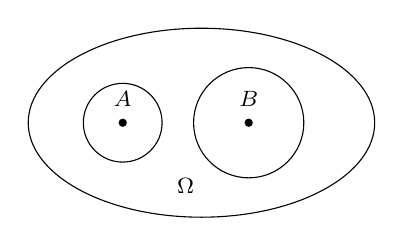
\begin{tikzpicture}[scale=1, font=\footnotesize, line join=round, line 
	cap=round, >=stealth]
	\path 
	(1.6,0) coordinate (B)
	(0,0) coordinate (A)
	(1,0) coordinate (C)
	;
	\draw (A) circle (0.5cm);
	\draw (B) circle (0.7cm);
	\draw (C) ellipse (2.2cm and 1.2cm) ;
	\draw (0.8,-0.8) node{$\Omega$};
	\foreach \p/\r in {A/90,B/90}
	\fill (\p) circle (1.5pt) node[shift={(\r:3mm)}]{$\p$};
	\end{tikzpicture}}
	\end{boxdn}
	\subsubsection{Biến cố độc lập}
	\begin{boxdn}
	Hai biến cố $A$ và $B$ được gọi là {\bf \textit{độc lập}} nếu việc xảy ra hay không xảy ra của biến cố này không làm ảnh hưởng tới xác suất xảy ra của biến cố kia.
	\end{boxdn}
	\begin{nx}
	Nếu hai biến cố $A$ và $B$ độc lập thì $\bar{A}$ và $B ; A$ và $\bar{B} ; \bar{A}$ và $\bar{B}$ cũng độc lập.
	\end{nx}	
	\subsubsection{Quy tắc nhân xác suất của hai biến cố độc lập}
	\begin{boxdn}
	Nếu hai biến cố $A$ và $B$ độc lập thì
	$$P(A B)=P(A) P(B).$$
	\end{boxdn}
	\begin{note}
	Từ quy tắc nhân xác suất ta thấy, nếu $P(A B) \neq P(A) P(B)$ thì hai biến cố $A$ và $B$ không độc lập.
	\end{note}
	\subsubsection{Biến cố hợp}
\begin{boxdn}
	{Cho hai biến cố $A$ và $B$. Biến cố \lq\lq $A$ hoặc $B$ xảy ra\rq\rq, kí hiệu là $A\cup B$ được gọi là \textbf{\textit{biến cố hợp}} của $A$ và $B$}
\end{boxdn}
\begin{note}
	{Biến cố $A \cup B$ xảy ra khi có ít nhất một trong hai biến cố $A$ và $B$ xảy ra. Tập hợp mô tả biến cố $A \cup B$ là hợp của hai tập hợp mô tả biến cố $A$ và biến cố $B$.}
\end{note}
\subsubsection{Quy tắc cộng xác suất}
\paragraph{Quy tắc cộng cho hai biến cố xung khắc}
\begin{boxdn}
	{Cho hai biến cố xung khắc $A$ và $B$. Khi đó: $P(A \cup B)=P(A)+P(B)$.}
\end{boxdn}
\paragraph{Quy tắc cộng cho hai biến cố bất kì}
\begin{boxdn}
	{Cho hai biến cố $A$ và $B$. Khi đó $P(A \cup B)=P(A)+P(B)-P(A B)$.}
\end{boxdn}
\end{tomtat}
%=============
\subsection{Các dạng toán}
\begin{dang}{Biến cố hợp}
\end{dang}
%%==========Ví dụ 1
\begin{vd}%[1K8BR-3]
	Một hộp đựng $15$ tấm thẻ cùng loại được đánh số từ $1$ đến $15$. Rút ngẫu nhiên một tấm thẻ trong hộp. Gọi $E$ là biến cố \lq\lq  Số ghi trên tấm thẻ là số lẻ\rq\rq; $F$ là biến cố \lq\lq  Số ghi trên tấm thẻ là số nguyên tố\rq\rq.
	\begin{enumerate}
		\item Mô tả không gian mẫu.
		\item Nêu nội dung của biến cố hợp $G=E \cup F$. Hỏi $G$ là tập con nào của không gian mẫu?
	\end{enumerate}
	\loigiai{
		\begin{enumerate}
			\item Không gian mẫu $\Omega=\{1 ; 2 ; 3 ; 4 ; 5 ; 6 ; 7 ; 8 ; 9 ; 10 ; 11 ; 12 ; 13 ; 14 ; 15\}$.
			\item $E \cup F$ là biến cố \lq\lq  Số ghi trên tấm thẻ là số lẻ hoặc số nguyên tố\rq\rq.\\
			Ta có $E=\{1 ; 3 ; 5 ; 7 ; 9 ; 11 ; 13 ; 15\} ; F=\{2 ; 3 ; 5 ; 7 ; 11 ; 13\}$.\\
			Vậy $G=E \cup F=\{1 ; 2 ; 3 ; 5 ; 7 ; 9 ; 11 ; 13 ; 15\}$.
		\end{enumerate}
	}
\end{vd}
%%==========Ví dụ 2
\begin{vd}%[1K8BR-3]
	Một tổ trong lớp 11B có $4$ học sinh nữ là Hương, Hồng, Dung, Phương và $5$ học sinh nam là Sơn, Tùng, Hoàng, Tiến, Hải. Trong giờ học, giáo viên chọn ngẫu nhiên một học sinh trong tổ đó lên bảng để kiểm tra bài.\\
	Xét các biến cố sau:\\
	$H$: \lq\lq  Học sinh đó là một bạn nữ\rq\rq;\\
	$K$: \lq\lq  Học sinh đó có tên bắt đầu là chữ cái $\mathrm{H}$\rq\rq.
	\begin{enumerate}
		\item Mô tả không gian mẫu.
		\item Nêu nội dung của biến cố hợp $M=H \cup K$. Mỗi biến cố $H, K, M$ là tập con nào của không gian mẫu?
	\end{enumerate}
	\loigiai{
		\begin{enumerate}
			\item $\Omega=\{\text{Hương, Hồng, Dung, Phương, Sơn, Tùng, Hoàng, Tiến, Hải}\}$.
			\item $M=H \cup K$ là biến cố \lq\lq  Học sinh được chọn là một bạn nữ hoặc một bạn nam\rq\rq. \\
			Ta có $H=\{\text{Hương, Hồng, Dung, Phương}\}$;\\
			$K=\{\text{Sơn, Tùng, Hoàng, Tiến, Hải}\}$.\\
			Vậy $M=\Omega=\{\text{Hương, Hồng, Dung, Phương, Sơn, Tùng, Hoàng, Tiến, Hải}\}$.
		\end{enumerate}
	}
\end{vd}
\begin{dang}{Biến cố giao}
\end{dang}
%%==========Ví dụ 3
\begin{vd}%[1K8BR-2]
	Một tổ trong lớp 11C có $9$ học sinh. Phỏng vấn $9$ bạn này với câu hỏi: \lq\lq  Bạn có biết chơi môn thể thao nào trong hai môn này không?\rq\rq. Nếu biết thì đánh dấu X vào ô ghi tên môn thể thao đó, không biết thì để trống. Kết quả thu được như sau:
	\begin{center}
	\begin{tabular}{|c|c|c|}
	\hline
	\diagbox{Tên học sinh}{Môn thể thao} & Cầu lông & Bóng bàn \\
	\hline
	Bảo & X & \\
	\hline
	Đăng & X & X \\
	\hline
	Giang & & \\
	\hline
	Hoa & X & X \\
	\hline
	Long & & \\
	\hline
	Mai & X & X \\
	\hline
	Phúc & X & X \\
	\hline
	Tuấn & X & \\
	\hline
	Yến & & \\
	\hline
	\end{tabular}
	\end{center}
	Chọn ngẫu nhiên một học sinh trong tổ. Xét các biến cố sau:\\	
	$U$: \lq\lq  Học sinh được chọn biết chơi cầu lông\rq\rq;\\
	$V$: \lq\lq  Học sinh được chọn biết chơi bóng bàn\rq\rq.
	\begin{enumerate}
	\item Mô tả không gian mẫu.
	\item Nội dung của biến cố giao $T=U V$ là gì? Mối biến cố $U$, $V$, $T$ là tập con nào của không gian mẫu?
	\end{enumerate}
	\loigiai{
	\begin{enumerate}
	\item Không gian mẫu $\Omega=\{\text{Bảo; Đăng; Giang; Hoa; Long; Mai; Phúc; Tuấn; Yến} \}$.
	\item $T$ là biến cố \lq\lq  Học sinh được chọn biết chơi cả cầu lông và bóng bàn\rq\rq.\\	
	Ta có: $U=\{\text{Bảo; Đăng; Long; Phúc; Tuấn; Yến}\}$;\\ $V=\{\text{Giang ; Long; Phúc; Tuấn}\}$.\\
	Vậy $T=U \cap V=\{$Long; Phúc; Tuấn$\}$.
	\end{enumerate}
	}
\end{vd}
%%==========Ví dụ 4
\begin{vd}%[1K8BR-2]
	Một hộp đựng $25$ tấm thẻ cùng loại được đánh số từ $1$ đến $25$. Rút ngẫu nhiên một tấm thẻ trong hộp. Xét các biến cố $P$ : \lq\lq  Số ghi trên tấm thẻ là số chia hết cho $4$\rq\rq; $Q$: \lq\lq  Số ghi trên tấm thẻ là số chia hết cho $6$\rq\rq.
	\begin{enumerate}
	\item Mô tả không gian mẫu.
	\item Nội dung của biến cố giao $S=P Q$ là gì? Mỗi biến cố $P$, $Q$, $S$ là tập con nào của không gian mẫu?
	\end{enumerate} 
	\loigiai{
	\begin{enumerate}
	\item $\Omega=\{1,2,3,4,5,6,7,8,9,10,11,12,13,14,15,16,17,18,19,20,21,22,23,24,25\}$.
	\item $S$ là biến cố \lq\lq  Số ghi trên tấm thẻ là số chia hết cho $4$ và chia hết cho $6$\rq\rq.\\	
	Ta có: $P=\{4,8,12,16,20,24\}$; $Q=\{6,12,18,24\}$.\\
	Vậy $T=P \cap Q=\{12;24\}$.
	\end{enumerate} 
	}
\end{vd}
\begin{dang}{Biến cố xung khắc}
\end{dang}
\begin{vd}%[1K8BS-1]
	Gieo đồng thời hai con xúc xắc cân đối, đồng chất. Xét các biến cố sau:\\
	$A$: \lq\lq  Tổng số chấm xuất hiện trên hai con xúc xắc lớn hơn hoặc bằng $7$\rq\rq;\\
	$B$: \lq\lq  Tổng số chấm xuất hiện trên hai con xúc xắc nhỏ hơn hoặc bằng $4$\rq\rq;\\
	$C$: \lq\lq  Tổng số chấm xuất hiện trên hai con xúc xắc là số nguyên tố\rq\rq.\\
	Trong các cặp biến cố $A$ và $B; \, A$ và $C; \, B$ và $C$, cặp biến cố nào xung khắc? Tại sao?
	\loigiai{
	Cặp biến cố $A$ và $B$ là xung khắc vì $A$ và $B$ không đồng thời xảy ra.\\
	Cặp biến cố $A$ và $C$ không xung khắc vì nếu tổng số chấm xuất hiện trên hai con xúc xắc bằng $7$ thì cả $A$ và $C$ xảy ra.\\
	Cặp biến cố $B$ và $C$ không xung khắc vì nếu tổng số chấm xuất hiện trên hai con xúc xắc bằng $3$ thì cả $B$ và $C$ xảy ra.
	}
\end{vd}
\begin{vd}
	Gieo hai con xúc xắc cân đối và đồng chất. Gọi $A$ là biến cố \lq\lq  Tổng số chấm xuất hiện trên hai con xúc xắc bằng 5\rq\rq, gọi $B$ là biến cố \lq\lq  Xuất hiện hai mặt có cùng số chấm\rq\rq. Hai biến cố $A$ và $B$ có thể đồng thời cùng xảy ra không?
	\loigiai{
	\begin{itemize}
	\item Biến cố $A=\{(1 ; 4) ;(4 ; 1) ;(2 ; 3) ;(3 ; 2)\}$.
	\item Biến cố $B=\{(1 ; 1) ;(2 ; 2) ;(3 ; 3) ;(4 ; 4);(5;5);(6;6)\}$.\\
	Hai biến cố $A$ và $B$ không thể đồng thời cùng xảy ra, chúng là 2 biến cố xung khắc.
	\end{itemize}
	}
\end{vd}
\begin{vd}
	Một hộp có $5$ viên bi xanh, $4$ viên bi đỏ và $2$ viên bi vàng. Lấy ra ngẫu nhiên đồng thời $2$ viên bi từ hộp. Hãy xác định các cặp biến cố xung khắc trong các biến cố sau:\\
	$A$ : \lq\lq  Hai viên bi lấy ra cùng màu xanh\rq\rq;\\
	$B$ : \lq\lq  Hai viên bi lấy ra cùng màu đỏ\rq\rq;\\
	$C$ : \lq\lq  Hai viên bi lấy ra cùng màu\rq\rq;\\
	$D$ : \lq\lq  Hai viên bi lấy ra khác màu\rq\rq.
	\loigiai{
	\begin{enumerate}
	\item Ta có hai biến cố $A$ và $B$ xung khắc.
	\item Biến cố $C$ xảy ra khi lấy ra 2 viên bi xanh hoặc 2 viên bi đỏ hoặc 2 viên bi vàng. Khi lấy được 2 viên bi màu xanh thì biến cố $A$ và biến cố $C$ cùng xảy ra. Khi lấy được 2 viên bi màu đỏ thì biến cố $B$ và biến cố $C$ cùng xảy ra. Do đó biến cố $C$ không xung khắc với biến cố $A$ và biến cố $B$.
	\item Biến cố $D$ xảy ra khi lấy ra 1 viên bi xanh, 1 viên bi đỏ; hoặc 1 viên bi xanh, 1 viên bi vàng; hoặc 1 viên bi đỏ, 1 viên bi vàng. Do đó biến cố $D$ xung khắc với biến cố $A$, xung khắc với biến cố $B$ và xung khắc với biến cố $C$.
	\end{enumerate}
	Vậy có 4 cặp biến cố xung khắc là: $A$ và $B ; A$ và $D ; B$ và $D ; C$ và $D$.
	}
\end{vd}
\begin{vd}
	Gieo hai con xúc xắc cân đối và đồng chất. Gọi $A$ là biến cố \lq\lq  Tổng số chấm xuất hiện trên hai con xúc xắc bằng 5\rq\rq, $B$ là biến cố \lq\lq  Tích số chấm xuất hiện trên hai con xúc xắc bằng 6\rq\rq. Gọi $C$ là biến cố \lq\lq  Có ít nhất một con xúc xắc xuất hiện mặt $1$ chấm\rq\rq.
	Hãy tìm một biến cố khác rỗng và xung khắc với cả ba biến cố $A, B$ và $C$.
	\loigiai{
	Biến cố $E$ : \lq\lq  Gieo 2 con xúc xắc có số chấm giống nhau và tổng số chấm lớn hơn 2\rq\rq.
	}
\end{vd}
\begin{vd}
	\indent
	\begin{enumerate}
	\item Hai biến cố đối nhau có xung khắc với nhau không?
	\item Hai biến cố xung khắc có phải là hai biến cố đối nhau không?
	\end{enumerate}
	\loigiai{
	\begin{enumerate}
	\item Hai biến cố đối nhau có xung khắc với nhau.
	\item Hai biến cố xung khắc chưa phải là hai biến cố đối nhau.
	\end{enumerate}
	}
\end{vd}
\begin{dang}{Biến cố độc lập}
\end{dang}
%%==========Ví dụ 5
\begin{vd}%[1K8KR-3]
	Một hộp đựng $4$ viên bi màu đỏ và $5$ viên bi màu xanh, có cùng kích thước và khối lượng.
	\begin{enumerate}
	\item Bạn Minh lấy ngẫu nhiên một viên bi, ghi lại màu của viên bi được lấy ra rồi trả lại viên bi vào hộp. Tiếp theo, bạn Hùng lấy ngẫu nhiên một viên bi từ hộp đó. Xét hai biến cố sau:\\	
	$A$: \lq\lq  Minh lấy được viên bi màu đỏ\rq\rq;\\	
	$B$: \lq\lq  Hùng lấy được viên bi màu xanh\rq\rq.\\	
	Chứng tỏ rằng hai biến cố $A$ và $B$ độc lập.
	\item Bạn Sơn lấy ngẫu nhiên một viên bi và không trả lại vào hộp. Tiếp theo, bạn Tùng lấy ngẫu nhiên một viên bi từ hộp đó. Xét hai biến cố sau:\\	
	$C$: \lq\lq  Sơn lấy được viên bi màu đỏ\rq\rq;\\	
	$D$: \lq\lq  Tùng lấy được viên bi màu xanh\rq\rq.\\	
	Chứng tỏ rằng hai biến cố $C$ và $D$ không độc lập.
	\end{enumerate}
	\loigiai{
	\begin{enumerate}
	\item Nếu $A$ xảy ra, tức là Minh lấy được viên bi màu đỏ. Vì Minh trả lại viên bi đã lấy vào hộp nên trong hộp có $4$ viên bi màu đỏ và $5$ viên bi màu xanh. Vậy $P(B)=\dfrac{5}{9}$.\\	
	Nếu $A$ không xảy ra, tức là Minh lấy được viên bi màu xanh. Vì Minh trả lại viên bi đã lấy vào hộp nên trong hộp vẫn có $4$ viên bi màu đỏ và $5$ viên bi màu xanh. Vậy $P(B)=\dfrac{5}{9}$.\\	
	Như vậy, xác suất xảy ra của biến cố $B$ không thay đổi bởi việc xảy ra hay không xảy ra của biến cố $A$.\\	
	Vì Hùng lấy sau Minh nên $P(A)=\dfrac{4}{9}$ dù biến cố $B$ xảy ra hay không xảy ra.\\	
	Vậy $A$ và $B$ độc lập.
	\item Nếu $C$ xảy ra, tức là Sơn lấy được viên bi màu đỏ. Vì Sơn không trả lại viên bi đó vào hộp nên trong hộp có $8$ viên bi với $3$ viên bi màu đỏ và $5$ viên bi màu xanh. Vậy $P(D)=\dfrac{5}{8}$. \\
	Nếu $C$ không xảy ra, tức là Sơn lấy được viên bi màu xanh. Vì Sơn không trả lại viên bi đã lấy vào hộp nên trong hộp có $4$ viên bi màu đỏ và $4$ viên bi màu xanh. Vậy $P(D)=\dfrac{4}{8}$. \\
	Như vậy, xác suất xảy ra của biến cố $D$ đã thay đổi phụ thuộc vào việc biến cố $C$ xảy ra hay không xảy ra. Do đó, hai biến cố $C$ và $D$ không độc lập.
	\end{enumerate}
	}
\end{vd}
%%%%%%%%%%%%%%%
\begin{dang}{Công thức cộng xác suất cho hai biến cố xung khắc}
\end{dang}
\begin{vd}%[1K8BS-1]%[1K8BS-3]
	Một hộp đựng $9$ tấm thẻ cùng loại được ghi số từ $1$ đến $9$. Rút ngẫu nhiên đồng thời hai tấm thẻ từ trong hộp. Xét các biến cố sau:\\
	$A$: \lq\lq  Cả hai tấm thẻ đều ghi số chẵn\rq\rq;\\
	$B$: \lq\lq  Chỉ có một tấm thẻ ghi số chẵn\rq\rq;\\
	$C$: \lq\lq  Tích hai số ghi trên hai tấm thẻ là một số chẵn\rq\rq.
	\begin{enumEX}{2}
	\item Chứng minh rằng $C=A \cup B$.
	\item Tính $\mathrm{P}(C)$.
	\end{enumEX}
	\loigiai{
	\begin{enumEX}{1}
	\item Biến cố $C$ xảy ra khi và chỉ khi trong hai tấm thẻ có ít nhất một tấm thẻ ghi số chẵn. Nếu cả hai tấm thẻ ghi số chẵn thì biến cố $A$ xảy ra. Nếu chỉ có một tấm thẻ ghi số chẵn thì biến cố $B$ xảy ra. Vậy $C$ là biến cố hợp của $A$ và $B$.
	\item Hai biến cố $A$ và $B$ là xung khắc. Do đó $\mathrm{P}(C)=\mathrm{P}(A \cup B)=\mathrm{P}(A)+\mathrm{P}(B)$.\\
	Ta cần tính $\mathrm{P}(A)$ và $\mathrm{P}(B)$.
	Không gian mẫu $\Omega$ là tập hợp tất cả các tập con có hai phần tử của tập $\{1 ; 2 ; \ldots ; 9\}$. Do đó $n(\Omega)=\mathrm{C}_{9}^{2}=36$. \\
	Tính $\mathrm{P}(A)$: Biến cố $A$ là tập hợp tất cả các tập con có hai phần tử của tập $\{2 ; 4 ; 6 ; 8\}$. Do đó $n(A)=\mathrm{C}_{4}^{2}=6$. Suy ra $\mathrm{P}(A)=\dfrac{n(A)}{n(\Omega)}=\dfrac{6}{36}$.\\
	Tính $\mathrm{P}(B)$ : Mỗi phần tử của $B$ được hình thành từ hai công đoạn: 
	\begin{itemize}
	\item Công đoạn 1: Chọn một số chẵn từ tập $\{2 ; 4 ; 6 ; 8\}$. Có $4$ cách chọn. 
	\item Công đoạn 2: Chọn một số lẻ từ tập $\{1 ; 3 ; 5 ; 7 ; 9\}$. Có $5$ cách chọn.
	\end{itemize}
	Theo quy tắc nhân, tập $B$ có $4 \cdot 5=20$ (phần tử). \\
	Do đó $n(B)=20$. Suy ra $\mathrm{P}(B)=\dfrac{n(B)}{n(\Omega)}=\dfrac{20}{36}$.\\
	Vậy $\mathrm{P}(C)=\mathrm{P}(A)+\mathrm{P}(B)=\dfrac{6}{36}+\dfrac{20}{36}=\dfrac{26}{36}=\dfrac{13}{18}$.
	\end{enumEX}
	}
\end{vd}
\begin{vd}%[1T9K2-4]
	Một đội tình nguyện gồm 9 học sinh khối 10 và 7 học sinh khối 11. Chọn ra ngẫu nhiên 3 người trong đội. Tính xác suất của biến cố \lq\lq  Cả 3 người được chọn học cùng một khối\rq\rq.
	\loigiai{
	Gọi $A$ là biến cố \lq\lq  Cả 3 học sinh được chọn đều thuộc khối 10 \rq\rq và $B$ là biến cố \lq\lq  Cả 3 học sinh được chọn đều thuộc khối 11\rq\rq. Khi đó $A \cup B$ là biến cố \lq\lq  Cả 3 người được chọn học cùng một khối\rq\rq. Do $A$ và $B$ là hai biến cố xung khắc nên $P(A \cup B)=P(A)+P(B)$.\\
	Ta thấy $P(A)=\dfrac{\mathrm{C}_9^3}{\mathrm{C}_{16}^3}$ và $P(B)=\dfrac{\mathrm{C}_7^3}{C_{16}^3}$, nên $P(A \cup B)=\dfrac{\mathrm{C}_9^3+\mathrm{C}_7^3}{\mathrm{C}_{16}^3}=\dfrac{17}{80}$.
	}
\end{vd}
\begin{dang}{Công thức cộng xác suất cho 2 biến cố bất kì}
\end{dang}
\begin{vd}%[1K8BS-3]
	Ở một trường trung học phổ thông $X$, có $19 \%$ học sinh học khá môn Ngữ văn, $32 \%$ học sinh học khá môn Toán, $7 \%$ học sinh học khá cả hai môn Ngữ văn và Toán. Chọn ngẫu nhiên một học sinh của trường $X$. Xét hai biến cố sau:\\
	$A$: \lq\lq  Học sinh đó học khá môn Ngữ văn\rq\rq;\\
	$B$: \lq\lq  Học sinh đó học khá môn Toán\rq\rq.
	Hãy tính tỉ lệ học sinh học khá môn Ngữ văn hoặc học khá môn Toán của trường $X$.
	\loigiai{
	Theo đề bài, ta có
	$$
	\mathrm{P}(A)=19 \%=0,19 ; \mathrm{P}(B)=32 \%=0,32 \text { và } \mathrm{P}(A B)=7 \%=0,07 \text {. }
	$$
	Theo công thức cộng xác suất, ta có
	$$
	\mathrm{P}(A \cup B)=\mathrm{P}(A)+\mathrm{P}(B)-\mathrm{P}(A B)=0{,}19+0{,}32-0{,}07=0{,}44 .
	$$
	Do đó, xác suất để chọn ngẫu nhiên một học sinh của trường $X$ học khá môn Ngữ văn hoặc học khá môn Toán là $0{,}44$.\\
	Vậy tỉ lệ học sinh học khá môn Ngữ văn hoặc học khá môn Toán của trường $X$ là $44 \%$.
	}
\end{vd}
\begin{vd}%[1T9K2-4]
	Một hộp chứa 100 tấm thẻ cùng loại được đánh số lần lượt từ 1 đến 100. Chọn ngẫu nhiên 1 thẻ từ hộp. Tính xác suất của biến cố \lq\lq  Số ghi trên thẻ được chọn chia hết cho 3 hoặc 5\rq\rq.
	\loigiai{
	Gọi $A$ là biến cố \lq\lq  Số ghi trên thẻ được chọn chia hết cho 3\rq\rq và $B$ là biến cố \lq\lq  Số ghi trên thẻ được chọn chia hết cho 5\rq\rq.\\
	$A \cup B$ là biến cố \lq\lq  Số ghi trên thẻ được chọn chia hết cho 3 hoặc 5\rq\rq.\\
	Từ 1 đến 100 có 33 số chia hết cho 3 nên $P(A)=\dfrac{33}{100}=0,33$.\\
	Từ 1 đến 100 có 20 số chia hết cho 5 nên $P(B)=\dfrac{20}{100}=0,2$.\\
	Một số chia hết cho cả 3 và 5 khi nó chia hết cho 15. Từ 1 đến 100 có 6 số chia hết cho 15 nên\\
	\centerline{$P(A B)=\dfrac{6}{100}=0,06$}.\\
	Vậy $P(A \cup B)=P(A)+P(B)-P(A B)=0,33+0,2-0,06=0,47$.
	}
\end{vd}
%=====================

\begin{dang}{Công thức nhân xác suất cho hai biến cố độc lập}
\end{dang}
\begin{vd}%[1K8BR-1] 
	Tại vòng chung kết của một đại hội thể thao, vận động viên An thi đấu môn Bắn súng, vận động viên Bình thi đấu môn Bơi lội.
	Biết rằng xác suất giành huy chương của vận động viên An và vận động viên Bình tương ứng là 0,8 và 0,9 . Hỏi xác suất để cả hai vận động viên đạt huy chương là bao nhiêu?
	\\Gọi $A$ là biến cố \lq\lq  Vận động viên An đạt huy chương\rq\rq; $B$ là biến cố \lq\lq  Vận động viên Bình đạt huy chương\rq\rq.
	\begin{enumEX}{1}
	\item Giải thích tại sao hai biến cố $A$ và $B$ là độc lập.
	\item Tính xác suất để cả hai vận động viên đạt huy chương.
	\item Sử dụng sơ đồ hình cây, tính xác suất để:
	\begin{enumerate}[--]
	\item Cả hai vận động viên không đạt huy chương;
	\item Vận động viên An đạt huy chương, vận động viên Bình không đạt huy chương;
	\item Vận động viên An không đạt huy chương, vận động viên Bình đạt huy chương.
	\end{enumerate}
	\end{enumEX}
	\loigiai{
	\begin{enumEX}{1}
	\item Vì hai vận động viên An và Bình thi đấu hai môn thể thao khác nhau nên hai biến cố $A$ và $B$ là độc lập.
	\item Vì $A$ và $B$ là hai biến cố độc lập nên áp dụng công thức nhân xác suất, ta có$$
	P(A B)=P(A) P(B)=0{,}8 \cdot 0{,}9=0{,}72 .
	$$
	\item \immini{Ta dùng sơ đồ hình cây để mô tả như hình bên.\\Theo sơ đồ hình cây, ta có
	$$
	\begin{aligned}
	& P(\bar{A} \bar{B})=0{,}2 \cdot 0{,}1=0{,}02 \\
	& P(A \bar{B})=0{,}8 \cdot 0{,}1=0{,}08 \\
	& P(\bar{A} B)=0{,}2 \cdot 0{,}9=0{,}18 .
	\end{aligned}
	$$}{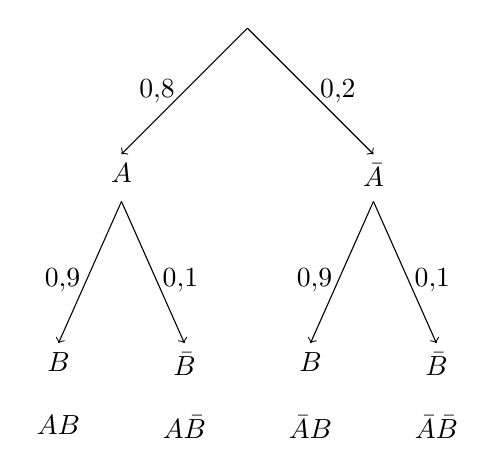
\begin{tikzpicture}[scale=.8]
	\coordinate [label=below:$A$](A) at (-2,-2);
	\coordinate [label=below:$\bar{A}$](B) at (2,-2);
	\coordinate [label=below:$B$](C) at (-3,-5);
	\coordinate [label=below:$\bar{B}$](D) at (-1,-5);
	\coordinate [label=below:$B$](E) at (1,-5);
	\coordinate [label=below:$\bar{B}$](F) at (3,-5);
	\draw[->](0,0)--(A);
	\draw[->](0,0)--(B);
	\draw[->](-2,-2.75)--(C);
	\draw[->](-2,-2.75)--(D);
	\draw[->](2,-2.75)--(E);
	\draw[->](2,-2.75)--(F);
	\coordinate [label=below:$AB$](G) at (-3,-6);
	\coordinate [label=below:$A\bar{B}$](H) at (-1,-6);
	\coordinate [label=below:$\bar{A} B$](I) at (1,-6);
	\coordinate [label=below:$\bar{A}\bar{B}$](J) at (3,-6);
	\draw (-1,-1) node[left] {$0{,}8$};
	\draw (1,-1) node[right] {$0{,}2$};
	\draw (-2.5,-4) node[left] {$0{,}9$};
	\draw (-1.5,-4) node[right] {$0{,}1$};
	\draw (1.5,-4) node[left] {$0{,}9$};
	\draw (2.5,-4) node[right] {$0{,}1$};
	\end{tikzpicture}}
	\end{enumEX}}
\end{vd}
\begin{vd}
	Các học sinh lớp 11D làm thí nghiệm gieo hai loại hạt giống $A$ và $B$. Xác suất để hai loại hạt giống $A$ và $B$ nảy mầm tương ứng là $0{,}92$ và $0{,}88$. Giả sử việc nảy mầm của hạt $A$ và hạt $B$ là độc lập với nhau. Dùng sơ đồ hình cây, tính xác suất để:
	\begin{enumEX}[\hspace*{.5cm}a)]{1}
	\item Hạt giống $A$ nảy mầm còn hạt giống $B$ không nảy mầm;
	\item Hạt giống $A$ không nảy mầm còn hạt giống $B$ nảy mầm;
	\item Ít nhất có một trong hai loại hạt giống nảy mầm.
	\end{enumEX}
	\loigiai{
	\begin{center}
	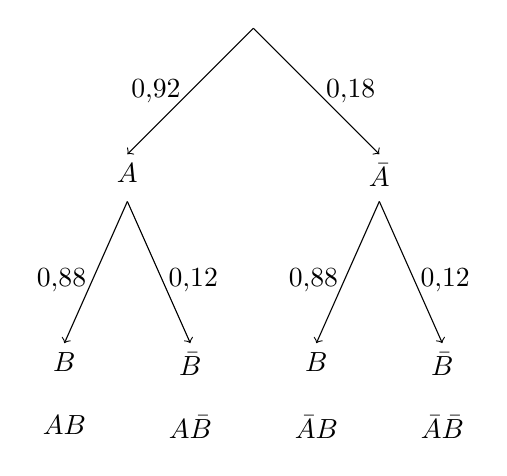
\begin{tikzpicture}[scale=.8]
	\coordinate [label=below:$A$](A) at (-2,-2);
	\coordinate [label=below:$\bar{A}$](B) at (2,-2);
	\coordinate [label=below:$B$](C) at (-3,-5);
	\coordinate [label=below:$\bar{B}$](D) at (-1,-5);
	\coordinate [label=below:$B$](E) at (1,-5);
	\coordinate [label=below:$\bar{B}$](F) at (3,-5);
	\draw[->](0,0)--(A);
	\draw[->](0,0)--(B);
	\draw[->](-2,-2.75)--(C);
	\draw[->](-2,-2.75)--(D);
	\draw[->](2,-2.75)--(E);
	\draw[->](2,-2.75)--(F);
	\coordinate [label=below:$AB$](G) at (-3,-6);
	\coordinate [label=below:$A\bar{B}$](H) at (-1,-6);
	\coordinate [label=below:$\bar{A} B$](I) at (1,-6);
	\coordinate [label=below:$\bar{A}\bar{B}$](J) at (3,-6);
	\draw (-1,-1) node[left] {$0{,}92$};
	\draw (1,-1) node[right] {$0{,}18$};
	\draw (-2.5,-4) node[left] {$0{,}88$};
	\draw (-1.5,-4) node[right] {$0{,}12$};
	\draw (1.5,-4) node[left] {$0{,}88$};
	\draw (2.5,-4) node[right] {$0{,}12$};
	\end{tikzpicture}
	\end{center}
	Gọi $A$ là biến cố \lq\lq  Hạt giống $A$ nảy mầm\rq\rq; $B$ là biến cố \lq\lq  Hạt giống $B$ nảy mầm\rq\rq.\\
	Vậy $\bar{A}$: \lq\lq  Hạt giống $A$ không nảy mầm\rq\rq; $\bar{B}$: \lq\lq  Hạt giống $B$ không nảy mầm\rq\rq.\\
	Vì hai biến cố $A$ và $B$ là độc lập với nhau nên
	\begin{enumEX}[\hspace*{.5cm}a)]{1}
	\item Áp dụng công thức nhân xác suất, ta có xác suất của biến cố \lq\lq  Hạt giống $A$ nảy mầm còn hạt giống $B$ không nảy mầm\rq\rq\, là$$
	P(A \cdot \bar{B})=P(A)\cdot P(\bar{B})=0{,}92 \cdot 0{,}12=0{,}1104 .
	$$
	\item Áp dụng công thức nhân xác suất, ta có xác suất của biến cố \lq\lq  Hạt giống $A$ không nảy mầm còn hạt giống $B$ nảy mầm\rq\rq\, là$$
	P(\bar{A} \cdot B)=P(\bar{A})\cdot P(B)=0{,}18 \cdot 0{,}88=0{,}1584 .
	$$
	\item Xác suất của biến cố $C$: \lq\lq  Ít nhất có một trong hai loại hạt giống nảy mầm\rq\rq\, là phần bù của biến cố \lq\lq  Cả hai loại hạt giống đều nảy mầm\rq\rq\,, ta có xác xuất $$
	P(C)=1-P(A)\cdot P(B)=0{,}92 \cdot 0{,}18=0{,}8244 .
	$$
	\end{enumEX}}
\end{vd}
\begin{vd}
	Cho $A$ và $B$ là hai biến cố độc lập. Biết $P(A)=0{,}6$ và $P(B)=0{,}8$. Hãy tính xác suất của các biến cố $A B, \bar{A} B$ và $\bar{A} \bar{B}$.
	\loigiai{
	Do $A$ và $B$ là hai biến cố độc lập nên
	$$P(A B)=P(A) P(B)=0{,}48.$$
	Vi $\bar{A}$ là biến cố đối của $A$ nên $P(\bar{A})=1-P(A)=0{,}4$. Do $\bar{A}$ và $B$ độc lập nên
	$$P(\bar{A} B)=P(\bar{A}) P(B)=0{,}32.$$
	Vì $\bar{B}$ là biến cố đối của $B$ nên $P(\bar{B})=1-P(B)=0{,}2$. Do $\bar{A}$ và $\bar{B}$ độc lập nên
	$$P(\bar{A} \bar{B})=P(\bar{A}) P(\bar{B})=0{,}08.	$$
	}
\end{vd}

\begin{dang}{Vận dụng}
\end{dang}
\begin{vd}%[1K8BT-3]%Ví dụ 2. 
	Số liệu thống kê tại một vùng cho thấy trong các vụ tai nạn ô tô có $0{,}37 \%$ người tử vong; $29 \%$ người không thắt dây an toàn và $0{,}28 \%$ người không thắt dây an toàn và tử vong. Chứng tỏ rằng việc không thắt dây an toàn khi lái xe và nguy cơ tử vong khi gặp tai nạn có liên quan với nhau.
	\loigiai{
	Chọn ngẫu nhiên một người đã bị tai nạn ô tô.\\
	Gọi $A$ là biến cố \lq\lq  Người đó đã tử vong\rq\rq; $B$ là biến cố \lq\lq  Người đó đã không thắt dây an toàn\rq\rq.
	\begin{note}
	Trong Mục 1 được sử dụng để phát hiện mối liên quan giữa hai biến cố.
	\end{note}
	Khi đó, $A B$ là biến cố \lq\lq  Người đó không thắt dây an toàn và đã tử vong\rq\rq. Ta có $$P(A)=0{,}37 \%=0{,}0037 ;\, P(B)=29 \%=0{,}29;$$ suy ra $P(A)\cdot P(B)=0{,}0037 \cdot 0{,}29=0{,}001073$. \\Mặt khác $P(A B)=0{,}28 \%=0{,}0028$.\\
	Vì $P(A B) \neq P(A) P(B)$ nên hai biến cố $A$ và $B$ không độc lập.\\
	Vậy việc không thắt dây an toàn khi lái xe có liên quan tới nguy cơ tử vong khi gặp tai nạn.}
\end{vd}
\begin{vd}
	Để nghiên cứu mối liên quan giữa thói quen hút thuốc lá với bệnh viêm phổi, nhà nghiên cứu chọn một nhóm 5000 người đàn ông. Với mỗi người trong nhóm, nhà nghiên cứu kiểm tra xem họ có nghiện thuốc lá và có bị viêm phổi hay không. Kết quả được thống kê trong bảng sau:
	\begin{center}
	\begin{tabular}{|c|c|c|}
	\hline & Viêm phổi & Không viêm phổi \\
	\hline Nghiện thuốc lá & 752 người & 1236 người \\
	\hline Không nghiện thuốc lá & 575 người & 2437 người \\
	\hline
	\end{tabular}
	\end{center}
	Từ bảng thống kê trên, hãy chứng tỏ rằng việc nghiện thuốc lá và mắc bệnh viêm phổi có liên quan với nhau.
	\loigiai{
	Gọi $A$ là biến cố \lq\lq  Người nghiện thuốc lá\rq\rq; $B$ là biến cố \lq\lq  Người mắc bệnh viêm phổi\rq\rq.\\
	Khi đó $AB$ là biến cố \lq\lq  Người nghiện thuốc là và mắc bệnh viêm phổi\rq\rq.\\
	Ta có $P(A)=\dfrac{752 + 1236}{5000}=0{,}3976$; $P(B)=\dfrac{752+575}{5000}=0{,}2654$.\\
	Suy ra $P(A)\cdot P(B)=0{,}10552304$.\\
	Mặt khác $P(AB)=\dfrac{752}{5000}=0{,}1504$.\\
	Vì $P(AB)\neq P(A)P(B)$ nên hai biến cố $A$ và $B$ không độc lập.\\
	Vậy việc nghiện thuốc lá và mắc bệnh viêm phổi có liên quan với nhau.}
\end{vd}
\begin{vd}
	Nguyệt và Nhi cùng tham gia bắn một cuộc thi bắn cung độc lập với nhau. Xác suất bắn trúng tâm bia của Nguyệt là $0{,}9$ và của Nhi là $0{,}8$. Tính xác suất để cả hai bạn cùng bắn trúng tâm bia.
	\loigiai{
	Xác suất bắn trúng tâm bia của Nguyệt là $P(A)=0{,}9$.\\
	Xác suất bắn trúng tâm bia của Nhi là $P(B)=0{,}8$.\\
	Xác suất để cả hai bạn cùng bắn trúng tâm bia là $P(AB)=P(A)P(B)=0{,}9\cdot 0{,}8=0{,}72$.
	}
\end{vd}
%----
\begin{vd}
	Hai bệnh nhân $X$ và $Y$ bị nhiễm vi rút SARS-CoV-2. Biết rằng xác suất bị biến chứng nặng của bệnh nhân $X$ là $0{,}1$ và của bệnh nhân $Y$ là $0{,}2$. Khả năng bị biến chứng nặng của hai bệnh nhân là độc lập.\\
	Hãy tính xác suất của các biến cố:
	\begin{enumerate}
	\item \lq\lq  Cả hai bệnh nhân đều bị biến chứng nặng\rq\rq;
	\item \lq\lq  Cả hai bệnh nhân đều không bị biến chứng nặng\rq\rq;
	\item \lq\lq  Bệnh nhân $X$ bị biến chứng nặng, bệnh nhân $Y$ không bị biến chứng nặng\rq\rq.
	\end{enumerate}
	\loigiai{
	Gọi $A$ là biến cố \lq\lq  Bệnh nhân $X$ bị biến chứng nặng\rq\rq. Ta có $P(A)=0{,}1$ và $P(\bar{A})=0{,}9$.\\
	Gọi $B$ là biến cố \lq\lq  Bệnh nhân $Y$ bị biến chứng nặng\rq\rq. Ta có $P(B)=0{,}2$ và $P(\bar{B})=0{,}8$.
	\begin{enumerate}
	\item \lq\lq  Cả hai bệnh nhân đều bị biến chứng nặng\rq\rq.\\
	Ta thấy $A$ và $B$ là hai biến cố độc lập nên xác suất cả hai bệnh nhân đều bị biến chứng nặng là
	$$	P(A B)=P(A) P(B)=0{,}02.$$
	\item \lq\lq  Cả hai bệnh nhân đều không bị biến chứng nặng\rq\rq.\\
	Do $\bar{A}$ và $\bar{B}$ độc lập nên xác suất cả hai bệnh nhân không bị biến chứng nặng là
	$$	P(\bar{A} \bar{B})=P(\bar{A}) P(\bar{B})=0{,}72.
	$$
	\item \lq\lq  Bệnh nhân $X$ bị biến chứng nặng, bệnh nhân $Y$ không bị biến chứng nặng\rq\rq.\\
	Do $A$ và $\bar{B}$ độc lập nên xác suất bệnh nhân $X$ bị biến chứng nặng, bệnh nhân $Y$ không bị biến chứng nặng là
	$$P(A \bar{B})=P(A) P(\bar{B})=0{,}08.$$
	\end{enumerate}
	Ta cũng có thể giải bài toán trên bằng cách sử dụng sơ đồ hình cây như sau:
	\begin{center}
	\begin{tikzpicture}[font=\footnotesize, line join=round, line cap=round, >=stealth,scale=1,rotate=-90]
	\path(0,0)node(a){Xác suất }
	++(2,4)node(b){$ X $ không bị biến chứng}
	(a)++(2,-4)node(c){$ X $ bị biến chứng}
	;
	\path
	(b)++(2,2)node(b1){$ Y $ bị biến chứng}
	(b)++(2,-2)node(b2){$ Y $ không bị biến chứng};
	\path (c)++(2,2)node(c1){$ Y $ bị biến chứng}
	(c)++(2,-2)node(c2){$ Y $ không bị biến chứng}
	;
	\path
	(b1)++(2,0)node[rectangle,draw=brown,text width=2cm,rounded 
	corners=2mm,align=center](b11){$ X $ không bị biến 
	chứng và $Y$ bị biến chứng}
	;
	\path
	(b2)++(2,0)node[rectangle,draw=brown,text width=2cm,rounded 
	corners=2mm,align=center](b21){$ X $ và 
	$Y$ không bị biến chứng};
	\path (c1)++(2,0)node[rectangle,draw=brown,text 
	width=2cm,rounded 
	corners=2mm,align=center](c11){$ X $ và $Y$ bị biến chứng};
	\path (c2)++(2,0)node[rectangle,draw=brown,text 
	width=2cm,rounded 
	corners=2mm,align=center](c21){$ X $ bị biến chứng và $Y$ 
	không 
	bị biến chứng};
	\draw[-stealth,teal,outer sep=0,inner 
	sep=0](a.south)--(b.north) node[pos=0.5,right]{$0{,}9$};
	\draw[-stealth,teal,outer sep=0,inner 
	sep=0](a.south)--(c.north) node[pos=0.5,left]{$0{,}1$};
	\draw[-stealth,teal,outer sep=0,inner 
	sep=0](b.south)--(b1.north) node[pos=0.5,right]{$0{,}2$};
	\draw[-stealth,teal,outer sep=0,inner 
	sep=0](b.south)--(b2.north) node[pos=0.5,left]{$0{,}8$};
	\draw[-stealth,teal,outer sep=0,inner 
	sep=0](c.south)--(c1.north) node[pos=0.5,right]{$0{,}2$};
	\draw[-stealth,teal,outer sep=0,inner 
	sep=0](c.south)--(c2.north)node[pos=0.5,left]{$0{,}8$};
	\draw[-stealth,teal,outer sep=0,inner 
	sep=0](b1.south)--(b11.north)node[pos=0.5,left]{$0{,}18$};
	\draw[-stealth,teal,outer sep=0,inner 
	sep=0](c1.south)--(c11.north)node[pos=0.5,left]{$0{,}02$};
	\draw[-stealth,teal,outer sep=0,inner 
	sep=0](b2.south)--(b21.north)node[pos=0.5,left]{$0{,}72$};
	\draw[-stealth,teal,outer sep=0,inner 
	sep=0](c2.south)--(c21.north)node[pos=0.5,left]{$0{,}08$};
	\end{tikzpicture}
	\end{center}
	Theo sơ đồ trên thì:
	\begin{enumerate}
	\item Xác suất cả hai bệnh nhân đều bị biến chứng nặng là $0{,}02$.
	\item Xác suất cả hai bệnh nhân không bị biến chứng nặng là $0{,}72$.
	\item Xác suất bệnh nhân $X$ bị biến chứng nặng, bệnh nhân $Y$ không bị biến chứng nặng là $0{,}08$.
	\end{enumerate}
	}
\end{vd}
%%%%%%%%%%%%%%%
%===========
\subsection{Bài tập rèn luyện}
\begin{bt}%[1T9B1-2]%[1T9Y1-2]
	Hộp thứ nhất chứa $3$ tấm thẻ cùng loại được đánh số lần lượt từ $1$ đến $3$. Hộp thứ hai chứa $5$ tấm thẻ cùng loại được đánh số lần lượt từ $1$ đến $5$. Lấy ra ngẫu nhiên từ mỗi hộp $1$ thẻ. Gọi $A$ là biến cố \lq\lq  Tổng các số ghi trên $2$ thẻ bằng $6$\rq\rq, $B$ là biến cố \lq\lq  Tích các số ghi trên $2$ thẻ là số lẻ\rq\rq. \\
	Hãy tìm một biến cố khác rỗng và xung khắc với cả hai biến cố $A$ và $B$.	
	\loigiai{
	Một biến cố khác rỗng và xung khắc với cả hai biến cố $A$ và $B$ là \\
	$C$ là biến cố \lq\lq  Tích các số ghi trên $2$ thẻ là số chẵn và tổng khác 6\rq\rq .\\
	Suy ra $C=\{(1;2);(1;4);(2;1);(2;2);(2;3);(2;5);(3;2);(3;4)\}$.
	}
\end{bt}
\begin{bt}%[1K8KS-3]%8.6. 
Một hộp đựng $8$ viên bi màu xanh và $6$ viên bi màu đỏ, có cùng kích thước và khối lượng. Bạn Sơn lấy ngẫu nhiên một viên bi từ hộp (lấy xong không trả lại vào hộp). Tiếp đó đến lượt bạn Tùng lấy ngẫu nhiên một viên bi từ hộp đó. Tính xác suất để bạn Tùng lấy được viên bi màu xanh.
\loigiai{
Tổng số bi trong hộp là $6+8=14$. Do đó số phần tử của không gian mẫu là $n(\Omega)=\mathrm{A}^2_{14}= 182$.\\
Gọi $A$ là biến cố: \lq\lq  Bạn Sơn lấy được viên bi màu xanh, sau đó Tùng lấy được viên bi màu xanh\rq\rq và $B$ là biến cố: \lq\lq  Bạn Sơn lấy được viên bi màu đỏ, sau đó Tùng lấy được viên bi màu xanh\rq\rq. \\
Suy ra $A\cup B$ là biến cố: \lq\lq  Bạn Sơn lấy ngẫu nhiên một viên bi từ hộp (lấy xong không trả lại vào hộp) và tiếp đó đến lượt bạn Tùng lấy ngẫu nhiên một viên bi từ hộp đó\rq\rq.\\
 $A$ và $B$ là hai biến cố xung khắc, vì Sơn không thể lấy một viên bi vừa màu xanh và vừa màu đỏ được. Suy ra 
 $\mathrm{P}(A\cup B)=\mathrm{P}(A)+\mathrm{P}(B)$.\\
Ta có $n(A)= 8 \cdot 7 =56 \Rightarrow \mathrm{P}(A)=\dfrac{n(A)}{n(\Omega)} = \dfrac{56}{182}$
và $n(B)= 6 \cdot 8 =48\Rightarrow \mathrm{P}(B)=\dfrac{n(B)}{n(\Omega)} = \dfrac{48}{182} $ .\\
$\Rightarrow \mathrm{P}(A\cup B)= \dfrac{56}{182}+\dfrac{48}{182} = \dfrac{104}{182}=\dfrac{4}{7}$.
}
\end{bt}
\begin{bt}%[1K8KS-3]%8.7. 
	Lớp $11A$ của một trường có $40$ học sinh, trong đó có $14$ bạn thích nhạc cổ điển, $13$ bạn thích nhạc trẻ và $5$ bạn thích cả nhạc cổ điển và nhạc trẻ. Chọn ngẫu nhiên một bạn trong lớp. Tính xác suất để:
	\begin{enumEX}{1}
	\item Bạn đó thích nhạc cổ điển hoặc nhạc trẻ;
	\item Bạn đó không thích cả nhạc cổ điển và nhạc trẻ.
	\end{enumEX}
	\loigiai{
	Gọi 	$A$ là biến cố: \lq\lq  Học sinh thích nhạc cổ điển\rq\rq;\\
	 	$B$ là biến cố: \lq\lq  Học sinh thích nhạc trẻ\rq\rq.\\
	Khi đó $A \cap B$ là biến cố: \lq\lq  Học sinh thích cả nhạc cổ điển và nhạc trẻ\rq\rq; \\
	$A \cup B$ là biến cố: \lq\lq  Học sinh hoặc thích nhạc cổ điển hoặc nhạc trẻ\rq\rq;\\
	$\overline{A \cup B}$ là biến cố: \lq\lq  Học sinh không thích cả nhạc cổ điển và nhạc trẻ\rq\rq.\\
	Ta có $n(A)=14,\, n(B)=13, \, n(A\cap B)=5$ và $n(\Omega) =40$. 
	\begin{enumEX}{1}
	\item Theo công thức cộng xác suất, ta có	
	\begin{align*}
	\mathrm{P}(A \cup B) &= \mathrm{P}(A) + \mathrm{P}(B) - \mathrm{P}(A \cap B) \\
	 &= \frac{n(A)}{n(\Omega)} + \frac{n(B)}{n(\Omega)} - \frac{n(A \cap B)}{n(\Omega)} \\
	&= \frac{14}{40} + \frac{13}{40} - \frac{5}{40} = \frac{22}{40} = 0{,}55.
	\end{align*}	
	Vậy xác suất để bạn chọn được một bạn thích nhạc cổ điển hoặc nhạc trẻ là $0{,}55$.	
	\item Theo tính chất xác suất đối lập, ta có	
$$\mathrm{P}(\overline{A \cup B}) = 1 - \mathrm{P}(A \cup B) = 1 - 0{,}55 = 0{,}45.$$	
	Vậy xác suất để bạn chọn được một bạn không thích cả nhạc cổ điển và nhạc trẻ là $0{,}45$.
	\end{enumEX}	
	}
\end{bt}
\begin{bt}%[1K8KS-3] %8.8. 
Một khu phố có $50$ hộ gia đình nuôi chó hoặc nuôi mèo, trong đó có $18$ hộ nuôi chó, $16$ hộ nuôi mèo và $7$ hộ nuôi cả chó và mèo. Chọn ngẫu nhiên một hộ trong khu phố trên. Tính xác suất để
\begin{enumEX}{1}
\item Hộ đó nuôi chó hoặc nuôi mèo;
\item Hộ đó không nuôi cả chó và mèo.
\end{enumEX}	
	\loigiai{
Gọi 	$A$ là biến cố: \lq\lq  Hộ gia đình nuôi chó\rq\rq;\\
$B$ là biến cố: \lq\lq  Hộ gia đình nuôi mèo\rq\rq.\\
Khi đó $A \cap B$ là biến cố: \lq\lq  Hộ gia đình nuôi cả chó và mèo\rq\rq; \\
$A \cup B$ là biến cố: \lq\lq  Hộ gia đình hoặc nuôi chó hoặc mèo\rq\rq;\\
$\overline{A \cup B}$ là biến cố: \lq\lq  Hộ gia đình không nuôi cả chó và mèo\rq\rq.\\
Ta có $n(A)=18,\, n(B)=16, \, n(A\cap B)=7$ và $n(\Omega) =50$. 
\begin{enumEX}{1}
	\item Theo công thức cộng xác suất, ta có	
	\begin{align*}
	\mathrm{P}(A \cup B) &= \mathrm{P}(A) + \mathrm{P}(B) - \mathrm{P}(A \cap B) \\
	&= \frac{n(A)}{n(\Omega)} + \frac{n(B)}{n(\Omega)} - \frac{n(A \cap B)}{n(\Omega)} \\
	&= \frac{18}{50} + \frac{16}{50} - \frac{7}{50} = \frac{27}{50} = 0{,}54.
	\end{align*}	
Vậy xác suất để chọn được một hộ gia đình nuôi chó hoặc nuôi mèo là $0{,}54$.
	\item Theo tính chất xác suất đối lập, ta có	
	$$	\mathrm{P}(\overline{A \cup B}) = 1 - \mathrm{P}(A \cup B) = 1 - \frac{7}{50} = \frac{43}{50} = 0{,}86.$$	
	Vậy xác suất để chọn được một hộ không nuôi cả chó và mèo là $0{,}86$.	
\end{enumEX}	
	}
\end{bt}
\begin{bt}%[1K8KS-3]%8.9. 
Một nhà xuất bản phát hành hai cuốn sách $A$ và $B$. Thống kê cho thấy có $50 \%$ người mua sách $A$; $70 \%$ người mua sách $B$; $30 \%$ người mua cả sách $A$ và sách $B$. Chọn ngẫu nhiên một người mua. Tính xác suất để:
\begin{enumEX}{1}
\item Người mua đó mua ít nhất một trong hai sách $A$ hoặc $B$;
\item Người mua đó không mua cả sách $A$ và sách $B$.
\end{enumEX}	
	\loigiai{
Gọi 	$A$ là biến cố: \lq\lq  Người mua mua sách $A$\rq\rq;\\
$B$ là biến cố: \lq\lq  Người mua mua sách $A$\rq\rq.\\
Khi đó $A \cap B$ là biến cố: \lq\lq  Người mua cả sách $A$ và sách $B$\rq\rq; \\
$A \cup B$ là biến cố: \lq\lq  Người mua ít nhất hoặc sách $A$ hoặc sách $B$\rq\rq;\\
$\overline{A \cup B}$ là biến cố: \lq\lq  Người mua không mua cả sách $A$ và sách $B$\rq\rq.\\
Ta có $	\mathrm{P}(A) = 0{,}5, \, \mathrm{P}(B) = 0{,}7, \, \mathrm{P}(A\cap B) = 0{,}3.$. 
\begin{enumEX}{1}
	\item Theo công thức cộng xác suất, ta có	
	\begin{align*}
	\mathrm{P}(A \cup B) &= \mathrm{P}(A) + \mathrm{P}(B) - \mathrm{P}(A \cap B) \\
	&= 0{,}5 + 0{,}7 - 0{,}3 = 0{,}9.
	\end{align*}	
Vậy xác suất người mua ít nhất một trong hai cuốn sách $A$ hoặc $B$ là $0.9$.
	\item Theo tính chất xác suất đối lập, ta có	
	$$	\mathrm{P}(\overline{A \cup B}) = 1 - \mathrm{P}(A \cup B) = 1 - 0{,}9 = 0{,}1.$$	
Vậy xác suất người không mua cả hai cuốn sách $A$ và $B$ là $0{,}1$.	
\end{enumEX}	
	}
\end{bt}
\begin{bt}%[1K8KS-3]%8.10. 
	Tại các trường trung học phổ thông của một tỉnh, thống kê cho thấy có $63 \%$ giáo viên môn Toán tham khảo bộ sách giáo khoa $A, 56 \%$ giáo viên môn Toán tham khảo bộ sách giáo khoa B và $28,5 \%$ giáo viên môn Toán tham khảo cả hai bộ sách giáo khoa A và $B$. Tính tỉ lệ giáo viên môn Toán các trường trung học phổ thông của tỉnh đó không tham khảo cả hai bộ sách giáo khoa $A$ và $B$.
	\loigiai{
	Gọi 	$A$ là biến cố: \lq\lq  Giáo viên môn Toán tham khảo bộ sách giáo khoa $A$\rq\rq;\\
	$B$ là biến cố: \lq\lq  Giáo viên môn Toán tham khảo bộ sách giáo khoa $B$\rq\rq.\\
	Khi đó $A \cap B$ là biến cố: \lq\lq  Giáo viên môn Toán tham khảo cả bộ sách giáo khoa $A$ và bộ sách giáo khoa $B$\rq\rq; \\
	$A \cup B$ là biến cố: \lq\lq  Giáo viên môn Toán tham khảo hoặc bộ sách giáo khoa $A$ hoặc bộ sách giáo khoa $B$\rq\rq.\\
	$\overline{A \cup B}$ là biến cố: \lq\lq  Giáo viên môn Toán không tham khảo cả bộ sách giáo khoa $A$ và bộ sách giáo khoa $B$\rq\rq.\\
	Ta có $	\mathrm{P}(A) = 0{,}63, \, \mathrm{P}(B) = 0{,}56, \, \mathrm{P}(A\cap B) = 0{,}285$. \\
	 Theo công thức cộng xác suất, ta có	
	\begin{align*}
	\mathrm{P}(A \cup B) &= \mathrm{P}(A) + \mathrm{P}(B) - \mathrm{P}(A \cap B) \\
	&= 0{,}63 + 0{,}56 - 0{,}285 = 0{,}905.
	\end{align*}	
 Theo tính chất xác suất đối lập, ta có	
	$$	\mathrm{P}(\overline{A \cup B}) = 1 - \mathrm{P}(A \cup B) = 1 - 0{,}905= 0{,}0905.$$
	Vậy tỉ lệ giáo viên môn Toán không tham khảo cả hai bộ sách giáo khoa $A$ và $B$ là $9{,}05 \%$.
	}
\end{bt}
\begin{bt}%[TeX hóa Sách 11 CD]%[Hoàng Khắc Ngân]%[1C5Y2-2]
	Trong hộp kín có $10$ quả bóng màu xanh và $8$ quả bóng màu đỏ, các quả bóng có kích thước và khối lượng giống nhau. Lấy ngẫu nhiên đồng thời $2$ quả bóng. Xét các biến cố:\\
	A: \lq\lq  Hai quả bóng lấy ra có màu xanh\rq\rq;\\
	B: \lq\lq  Hai quả bóng lấy ra có màu đỏ\rq\rq.\\
	Chọn phát biểu đúng trong những phát biểu sau đây?
	\begin{enumerate}
	\item Biến cố hợp của hai biến cố $A$ và $B$ là \lq\lq  Hai quả bóng lấy ra có cùng màu đỏ hoặc cùng màu xanh\rq\rq;
	\item Biến cố hợp của hai biến cố $A$ và $B$ là \lq\lq  Hai quả bóng lấy ra có màu khác nhau\rq\rq;
	\item Biến cố hợp của hai biến cố $A$ và $B$ là \lq\lq  Hai quả bóng lấy ra có cùng màu\rq\rq.
	\end{enumerate}
	\loigiai{
	\begin{enumerate}
	\item Phát biểu đúng;
	\item Phát biểu sai;
	\item Phát biểu đúng.
	\end{enumerate}
	}
\end{bt}
\begin{bt}%[TeX hóa Sách 11 CD]%[Hoàng Khắc Ngân]%[1C5Y2-1]
	Một hộp có $3$ quả bóng màu xanh, $4$ quả bóng màu đỏ; các quả bóng có kích thước và khối lượng như nhau. Lấy bóng ngẫu nhiên hai lần liên tiếp, trong đó mỗi lần lấy ngẫu nhiên một quả bóng trong hộp, ghi lại màu của quả bóng lấy ra và bỏ lại quả bóng đó vào hộp.\\
	Xét các biến cố:\\
	$A$: \lq\lq  Quả bóng màu xanh được lấy ra ở lần thứ nhất\rq\rq;\\
	$B$: \lq\lq  Quả bóng màu đỏ được lấy ra ở lần thứ hai\rq\rq.\\
	Hỏi hai biến cố $A$ và $B$ có độc lập không? Vì sao?
	\loigiai{
Trước hết, biến cố $B$ xảy ra sau biến cố $A$ nên việc xảy ra hay không xảy ra của biến cố $B$ không làm ảnh hưởng đến xác suất xảy ra của biến cố $A$.\\
	Mặt khác, ta có xác suất của biến cố $B$ khi biến cố $A$ xảy ra bằng $\dfrac{4}{7}$; xác suất của biến cố $B$ khi biến cố $A$ không xảy ra cũng bằng $\dfrac{4}{7}$.\\
	Do đó việc xảy ra hay không xảy ra của biến cố $A$ không làm ảnh hưởng đến xác suất xảy ra của biến cố $B$.\\
	Vậy hai biến cố $A$ và $B$ là độc lập.
}	
\end{bt}
%%%%%%%%%%%%%%
\begin{bt}
	Gieo hai con xúc xắc cân đối và đồng chất. Gọi $A$ là biến cố \lq\lq  Tổng số chấm xuất hiện trên hai con xúc xắc bằng 5\rq\rq, $B$ là biến cố \lq\lq  Tích số chấm xuất hiện trên hai con xúc xắc bằng 6\rq\rq.
	\begin{enumerate}
	\item Hãy viết tập hợp mô tả các biến cố trên.
	\item Hãy liệt kê các kết quả của phép thử làm cho cả hai biến cố $A$ và $B$ cùng xảy ra.
	\end{enumerate}
	\loigiai{
	\begin{enumerate}
	\item 	Biến cố $A=\{(1 ; 4) ;(4 ; 1) ;(2 ; 3) ;(3 ; 2)\}$.\\
	Biến cố $B=\{(1 ; 6) ;(6 ; 1) ;(2 ; 3) ;(3 ; 2)\}$.
	\item Kết quả của phép thử làm cho cả hai biến cố $A$ và $B$ cùng xảy ra là $\{(2 ; 3) ;(3 ; 2)\}$.
	\end{enumerate}
	}
\end{bt}
\begin{bt}
	Gieo hai con xúc xắc cân đối và đồng chất. Gọi $A$ là biến cố \lq\lq  Tổng số chấm xuất hiện trên hai con xúc xắc bằng 5\rq\rq, $B$ là biến cố \lq\lq  Tích số chấm xuất hiện trên hai con xúc xắc bằng 6\rq\rq. Gọi $C$ là biến cố \lq\lq  Có ít nhất một con xúc xắc xuất hiện mặt $1$ chấm\rq\rq. Hãy viết tập hợp mô tả các biến cố giao $AC$ và $BC$.
	\loigiai{
	Biến cố $A=\{(1 ; 4) ;(4 ; 1) ;(2 ; 3) ;(3 ; 2)\}$.\\
	Biến cố $B=\{(1 ; 6) ;(6 ; 1) ;(2 ; 3) ;(3 ; 2)\}$.\\
	Biến cố $C=\{(1 ; 6) ;(6 ; 1) ;(1 ; 5) ;(5 ; 1) ;(1 ; 4) ;(4 ; 1) ;(1 ; 3) ;(3 ; 1) ;(1 ; 2) ;(2 ; 1) ;(1 ; 1)\}$.\\
	Kết hợp tập hợp mô tả biến cố $A, B$ ở trên, ta có biến cố $AC=\{(1 ; 4) ;(4 ; 1)\};$ $B C=\{(1 ; 6) ;(6 ; 1)\}.$
	}
\end{bt}
\begin{bt}
	Gieo hai con xúc xắc cân đối và đồng chất. Gọi $A$ là biến cố \lq\lq  Tổng số chấm xuất hiện trên hai con xúc xắc bằng 5\rq\rq, $B$ là biến cố \lq\lq  Tích số chấm xuất hiện trên hai con xúc xắc bằng 6\rq\rq. Gọi $C$ là biến cố \lq\lq  Có ít nhất một con xúc xắc xuất hiện mặt $1$ chấm\rq\rq.
	\begin{enumerate}
	\item Gọi $D$ là biến cố \lq\lq  Số chấm xuất hiện trên con xúc xắc thứ nhất là 3\rq\rq. Hãy xác định các biến cố $AD$, $BD$ và $CD$.
	\item Gọi $\bar{A}$ là biến cố đối của biến cố $A$. Hãy viết tập hợp mô tả các biến cố giao $\bar{A}B$ và $\bar{A}C$.
	\end{enumerate}
	\loigiai{
	\begin{enumerate}
	\item Biến cố $D=\{(3 ; 1) ;(3 ; 2) ;(3 ; 3) ;(3 ; 4); (3 ; 5); (3 ; 6)\}$.\\
	Biến cố $AD=\{(3 ; 2)\}$.\\
	Biến cố $BD=\{(3 ; 2) \}$.\\
	Biến cố $CD=\{(3 ; 1) \}$.
	\item Gọi $\bar{A}$ là biến cố đối của biến cố $A$. \\
	Biến cố giao $\bar{A}B=\{(1 ; 6) ;(6 ; 1)\}$.\\
	Biến cố giao $\bar{A}C=\{(1 ; 6) ;(6 ; 1) ;(1 ; 5) ;(5 ; 1) ;(1 ; 3) ;(3 ; 1) ;(1 ; 2) ;(2 ; 1) ;(1 ; 1)\}$.
	\end{enumerate}
	}
\end{bt}
\begin{bt}%[Võ Hoàng Nghĩa]%[1T9B2-4]
	Một hộp chứa 5 viên bi xanh và 3 viên bi đỏ có cùng kích thước và khối lượng. Lấy ra ngẫu nhiên đồng thời 2 viên bi từ hộp. Gọi $A$ là biến cố \lq\lq  Hai viên bi lấy ra đều có màu xanh\rq\rq, $B$ là biến cố \lq\lq  Hai viên bi lấy ra đều có màu đỏ\rq\rq.
	\begin{enumerate}
	\item Có bao nhiêu kết quả thuận lợi cho biến cố $A$? Có bao nhiêu kết quả thuận lợi cho biến cố $B$?
	\item Hãy mô tả bằng lời biến cố $A \cup B$ và tính số kết quả thuận lợi cho biến cố $A \cup B$.
	\end{enumerate}
	\loigiai{
	\begin{enumerate}
	\item Số kết quả thuận lợi cho biến cố $A$ là $\mathrm{C}_5^2=10$. Số kết quả thuận lợi cho biến cố $B$ là $\mathrm{C}_3^2=3$.
	\item $A \cup B$ là biến cố \lq\lq  Hai viên bi lấy ra có cùng màu\rq\rq. Số kết quả thuận lợi cho biến cố $A \cup B$ là $\mathrm{C}_5^2+\mathrm{C}_3^2=13$.
	\end{enumerate}
	}
\end{bt}
\begin{bt}%[Võ Hoàng Nghĩa]%[1T9B2-2]
	Thực hiện hai thí nghiệm. Gọi $T_1$ và $T_2$ lần lượt là các biến cố \lq\lq  Thí nghiệm thứ nhất thành công\rq\rq và \lq\lq  Thí nghiệm thứ hai thành công\rq\rq. Hãy biểu diễn các biến cố sau theo hai biến cố $T_1$ và $T_2$.
	\begin{enumerate}
	\item $A$: \lq\lq  Có it nhất một trong hai thí nghiệm thành công\rq\rq.
	\item $B$: \lq\lq  Có đúng một trong hai thí nghiệm thành công\rq\rq.
	\end{enumerate}
	\loigiai{
	\begin{enumerate}
	\item $A=T_1 \cup T_2$.
	\item $B=\overline{T_1} T_2 \cup T_1 \bar{T}_2$.
	\end{enumerate}
	}
\end{bt}
%Bài 1
\begin{bt}%[TeX hóa Sách 11 CD]%[Hoàng Khắc Ngân]%[1C5Y2-2]
	Tung một đồng xu cân đối và đồng chất hai lần liên tiếp. Xét các biến cố:\\
	$A$: \lq\lq  Lần thứ nhất xuất hiện mặt ngửa\rq\rq;\\
	$B$: \lq\lq  Lần thứ hai xuất hiện mặt ngửa\rq\rq;\\
	$C$: \lq\lq  Cả hai lần đều xuất hiện mặt ngửa\rq\rq;\\
	$D$: \lq\lq  Có ít nhất một lần xuất hiện mặt ngử\rq\rq.\\
	Trong hai biến cố $C, D$, biến cố nào là biến cố hợp của hai biến cố $A, B$ ? Biến cố nào là biến cố giao của hai biến cố $A, B$?
	\loigiai{
	Biến cố $C$ là biến cố giao của hai biến cố $A, B$.\\
	Biến cố $D$ là biến cố hợp của hai biến cố $A, B$.
	}
\end{bt}
%Bài 2
\begin{bt}%[TeX hóa Sách 11 CD]%[Hoàng Khắc Ngân]%[1C5Y2-1]
	Gieo ngẫu nhiên một xúc xắc cân đối và đồng chất hai lần liên tiếp. Xét các biến cố:\\
	$A$: \lq\lq  Số chấm xuất hiện ở lần gieo thứ nhất lớn hơn 4\rq\rq ;\\
	$B$: \lq\lq  Số chấm xuất hiện ở lần gieo thứ hai nhỏ hơn 4\rq\rq ;\\
	$C$: \lq\lq  Số chấm xuất hiện ở lần gieo thứ nhất nhỏ hơn 4\rq\rq.\\
	Trong các biến cố trên, hãy tìm cặp biến cố độc lập.
	\loigiai{
	Cặp biến cố độc lập là $A, B$ và $B, C$.
	}
\end{bt}
\begin{bt}
	Trong hộp có 1 quả bóng xanh, 1 quả bóng đỏ, 1 quả bóng vàng. Lấy ra ngẫu nhiên 1 quả bóng, xem màu rồi trả lại hộp. Lặp lại phép thử trên 2 lần và gọi $A_k$ là biến cố quả bóng lấy ra lần thứ $k$ là bóng xanh $(k=1,2)$.
	\begin{enumerate}
	\item $A_1, A_2$ có là các biến cố độc lập không? Tại sao?
	\item Nếu trong mỗi phép thử trên ta không trả bóng lại hộp thì $A_1, A_2$ có là các biến cố độc lập không? Tại sao?
	\end{enumerate}
	\loigiai{
	\begin{enumerate}
	\item Nếu $A_1$ xảy ra thì sau khi trả lại quả bóng thứ nhất vào hộp, trong hộp có 1 quả bóng xanh, 1 quả bóng đỏ và 1 quả bóng vàng, do đó xác suất xảy ra $A_2$ là $\dfrac{1}{3}$.\\
	Ngược lại, nếu $A_1$ không xảy ra thì sau khi trả lại quả bóng thứ nhất vào hộp, trong hộp vẫn có 1 quả bóng xanh, 1 quả bóng đỏ và 1 quả bóng vàng, do đó xác suất xảy ra $A_2$ là $\dfrac{1}{3}$.\\
	Ta thấy khi $A_1$ xảy ra hay không xảy ra thì xác suất của biến cố $A_2$ luôn bằng $\dfrac{1}{3}$. Do quả bóng lấy ra lần thứ nhất được trả lại hộp nên biến cố $A_2$ xảy ra hay không xảy ra không ảnh hưởng đến xác suất xảy ra của $A_1$. \\
	Vậy $A_1$ và $A_2$ là hai biến cố độc lập.
	\item Giả sử quả bóng lấy ra lần đầu tiên không được trả lại hộp.\\
	Nếu $A_1$ xảy ra thì trước khi bốc quả bóng thứ hai, trong hộp có 1 quả bóng đỏ, 1 quả bóng vàng. Do đó xác suất xảy ra $A_2$ là $0$.\\
	Ngược lại, nếu $A_1$ không xảy ra thì trước khi bốc quả bóng thứ hai, trong hộp có 2 quả bóng,
	trong đó có đúng 1 quả bóng xanh. Do đó xác suất xảy ra $A_2$ là $\dfrac{1}{2}$.\\
	Ta thấy xác suất xảy ra của biến cố $A_2$ phụ thuộc vào sự xảy ra của $A_1$.\\
	Vậy $A_1$ và $A_2$ không là hai biến cố độc lập.
	\end{enumerate}
	}
\end{bt}
\begin{bt}
	Hãy chỉ ra 2 biến cố độc lập trong phép thử tung 2 đồng xu cân đối và đồng chất.
	\loigiai{
	Biến cố khi gieo 2 đồng xu có cùng mặt sấp; biến cố khi gieo 2 đồng xu có cùng mặt ngửa.
	}
\end{bt}
\begin{bt}%[1T9B1-4]%[1T9Y1-2]
	Một hộp chứa $21$ tấm thẻ cùng loại được đánh số từ $1$ đến $21$. Chọn ra ngẫu nhiên $1$ thẻ từ hộp. Gọi $A$ là biến cố \lq\lq  Số ghi trên thẻ được chọn chia hết cho $2$\rq\rq, $B$ là biến cố \lq\lq  Số ghi trên thẻ được chọn chia hết cho $3$\rq\rq.
	\begin{enumerate}
	\item Hãy mô tả bằng lời biến cố $A B$.
	\item Hai biến cố $A$ và $B$ có độc lập không? Tại sao?
	\end{enumerate}
	\loigiai{
	\begin{enumerate}
	\item $A$ là biến cố \lq\lq  Số ghi trên thẻ được chọn chia hết cho $2$\rq\rq $\,$nên $A=\{2;4;6;8;10;12;14;16;18;20\}$.\\
	$B$ là biến cố \lq\lq  Số ghi trên thẻ được chọn chia hết cho $3$\rq\rq $\,$nên $B=\{3;6;9;12;15;18;21\}$.\\
	Suy ra biến cố $AB=\{6;12;18\}$. \\
	Vậy biến cố $AB$ là \lq\lq  Số ghi trên thẻ được chọn chia hết cho 6\rq\rq.
	\item 
	Xác suất $P(A)=\dfrac{10}{21}$;	Xác suất $P(B)=\dfrac{7}{21}=\dfrac{1}{3}$; Xác suất $P(AB)=\dfrac{3}{21}=\dfrac{1}{7}$.\\
	Ta có $P(AB)=\dfrac{1}{7}\neq \dfrac{10}{21}\cdot \dfrac{1}{3}=\dfrac{10}{63}=P(A)P(B)$ nên hai biến cố $A$ và $B$ không độc lập.
	\end{enumerate}	
	}
\end{bt}
%%==========Bài 1
\begin{bt}%[1K8BR-2]
	Một hộp đựng $15$ tấm thẻ cùng loại được đánh số từ $1$ đến $15$. Rút ngẫu nhiên một tấm thẻ và quan sát số ghi trên thẻ. Gọi $A$ là biến cố \lq\lq  Số ghi trên tấm thẻ nhỏ hơn $7$\rq\rq; $B$ là biến cố \lq\lq  Số ghi trên tấm thẻ là số nguyên tố\rq\rq.
	\begin{enumerate}
	\item Mô tả không gian mẫu.
	\item Mỗi biến cố $A \cup B$ và $A B$ là tập con nào của không gian mẫu?
	\end{enumerate}
	\loigiai{
	\begin{enumerate}
	\item Khi rút 1 thẻ từ 15 thẻ được đánh số thì không gian mẫu là: \\
	$\Omega= \{1;2;3;4;5;6;7;8;9;10;11;12;13;14;15 \}$.
	\item 
	Các kết quả thuận lợi của biến cố $A$: $A= \{1;2;3;4;5;6 \}$.\\
	Các kết quả thuận lợi của biến cố $B$: $B=\{2;3;5;7;11;13 \}$.\\
	$A \cup B$ là biến cố \lq\lq  Số ghi trên thẻ nhỏ hơn $7$ hoặc số nguyên tố\rq\rq.\\
	$A \cup B = \{1;2;3;4;5;6;7;11;13 \}$.\\
	$AB$ là biến cố \lq\lq  Số ghi trên thẻ nhỏ hơn $7$ và nguyên tố\rq\rq.\\
	$AB=\{2;3;5 \}$.
	\end{enumerate}
	}
\end{bt}
%%==========Bài 2
\begin{bt}%[1K8KR-3]
	Gieo hai con xúc xắc cân đối, đồng chất. Xét các biến cố sau:\\
	$E$: \lq\lq  Số chấm xuất hiện trên hai con xúc xắc đều là số chẵn\rq\rq;\\
	$F$: \lq\lq  Số chấm xuất hiện trên hai con xúc xắc khác tính chẵn lẻ\rq\rq;\\
	$K$: \lq\lq  Tích số chấm xuất hiện trên hai con xúc xắc là số chẵn\rq\rq.\\
	Chứng minh rằng $K$ là biến cố hợp của $E$ và $F$.
	\loigiai{
	Để tích của số chấm xuất hiện trên hai con xúc xắc là số chẵn thì có 2 trường hợp xảy ra.\\
	TH1: 1 con xúc xắc xuất hiện mặt chẵn, con còn lại xuất hiện mặt lẻ.\\
	Khi đó số chấm xuất hiện trên hai con xúc xắc khác tính chẵn lẽ.\\
	TH2: 2 con xúc xắc xuất hiện mặt chẵn.\\
	Do đó $K$ là biến cố hợp của $E$ và $F$.
	}
\end{bt}
%%==========Bài 3
\begin{bt}%[1K8BR-3]
	Chọn ngẫu nhiên một học sinh trong trường em. Xét hai biến cố sau:\\
	$P$: \lq\lq  Học sinh đó bị cận thị\rq\rq;\\
	$Q$: \lq\lq  Học sinh đó học giỏi môn Toán\rq\rq.\\
	Nêu nội dung của các biến cố $P \cup Q$; $P Q$ và $\bar{P} \bar{Q}$.
	\loigiai{
	$P \cup Q$ là biến cố \lq\lq  Học sinh đó bị cận thị hoặc học sinh đó giỏi môn Toán\rq\rq.\\
	$PQ$ là biến cố \lq\lq  Học sinh đó bị cận thị và học giỏi môn Toán\rq\rq.\\
	$\bar{P}$ là biến cố \lq\lq  Học sinh đó không bị cận thị\rq\rq.\\
	$\bar{Q}$ là biến cố \lq\lq  Học sinh đó không giỏi môn Toán\rq\rq.\\
	$\bar{P} \bar{Q}$ là biến cố \lq\lq  Học sinh đó không bị cận và không giỏi môn Toán\rq\rq. 
	}
\end{bt}
%%==========Bài 4
\begin{bt}%[1K8KR-3]
	Có hai chuồng nuôi thỏ. Chuồng I có $5$ con thỏ đen và $10$ con thỏ trắng. Chuồng II có $3$ con thỏ trắng và $7$ con thỏ đen. Từ mỗi chuồng bắt ngẫu nhiên ra một con thỏ. Xét hai biến cố sau:\\
	$A$: \lq\lq  Bắt được con thỏ trắng từ chuồng I\rq\rq;\\
	$B$: \lq\lq  Bắt được con thỏ đen từ chuồng Il\rq\rq.\\
	Chứng tỏ rằng hai biến cố $A$ và $B$ độc lập.
	\loigiai{
	Nếu $A$ xảy ra, tức là bắt được con thỏ trắng ở chuồng I. Khi đó, số thỏ ở chuồng II không bị thay đổi và có $3$ thỏ trắng và $7$ thỏ đen. Vậy $P(B)=\dfrac{7}{10}$.\\	
	Nếu $A$ không xảy ra, tức là bắt được thỏ đen ở chuồng I.Khi đó, số thỏ ở chuồng II không bị thay đổi và có $3$ thỏ trắng và $7$ thỏ đen. Vậy $P(B)=\dfrac{7}{10}$.\\	
	Như vậy, xác suất xảy ra của biến cố $B$ không thay đổi bởi việc xảy ra hay không xảy ra của biến cố $A$.\\	
	Tương tự $P(A)=\dfrac{2}{3}$ dù biến cố $B$ xảy ra hay không xảy ra.\\	
	Vậy $A$ và $B$ độc lập.
	}
\end{bt}
%%==========Bài 5
\begin{bt}%[1K8KR-3]
	Có hai chuồng nuôi gà. Chuồng I có $9$ con gà mái và $3$ con gà trống. Chuồng II có $3$ con gà mái và $6$ con gà trống. Bắt ngẫu nhiên một con gà của chuồng I để đem bán rồi dồn các con gà còn lại của chuồng I vào chuồng II. Sau đó bắt ngẫu nhiên một con gà của chuồng II. Xét hai biến cố sau:\\
	$E$: \lq\lq  Bắt được con gà trống từ chuồng I\rq\rq;\\
	$F$: \lq\lq  Bắt được con gà mái từ chuồng II\rq\rq.\\
	Chứng tỏ rằng hai biến cố $E$ và $F$ không độc lập.
	\loigiai{
	Nếu $E$ xảy ra, tức là bắt được con gà trống từ chuồng I. Vì con gà trống bị bắt đem đi bán và số gà ở chuồng I dồn vô chuồng II, nên khi bắt gà mái từ chuồng II sẽ có $12$ gà mái và $8$ gà trống. Vậy $P(F)=\dfrac{12}{20}=\dfrac{3}{5}$. \\
	Nếu $E$ không xảy ra, tức là bắt được con gà mái từ chuồng I. Vì con gà mái bị bắt đem đi bán và số gà ở chuồng I dồn vô chuồng II, nên khi bắt gà mái từ chuồng II sẽ có $11$ gà mái và $9$ gà trống. Vậy $P(F)=\dfrac{11}{20}$. \\
	Như vậy, xác suất xảy ra của biến cố $F$ đã thay đổi phụ thuộc vào việc biến cố $E$ xảy ra hay không xảy ra. Do đó, hai biến cố $E$ và $F$ không độc lập.
	}
\end{bt}
%%%%%%%%%%%%%%%%
\begin{bt}%[1T9B1-2]%[1T9Y1-2]
	Hộp thứ nhất chứa $3$ tấm thẻ cùng loại được đánh số lần lượt từ $1$ đến $3$. Hộp thứ hai chứa $5$ tấm thẻ cùng loại được đánh số lần lượt từ $1$ đến $5$. Lấy ra ngẫu nhiên từ mỗi hộp $1$ thẻ. Gọi $A$ là biến cố \lq\lq  Tổng các số ghi trên $2$ thẻ bằng $6$\rq\rq, $B$ là biến cố \lq\lq  Tích các số ghi trên $2$ thẻ là số lẻ\rq\rq. 
	Hãy viết tập hợp mô tả biến cố $A B$ và tính $P(A B)$.
	\loigiai{
	\begin{enumerate}
	\item Hãy viết tập hợp mô tả biến cố $A B$ và tính $P(A B)$.\\
	Hộp thứ nhất chứa $3$ tấm thẻ cùng loại được đánh số $1; 2; 3$.\\
	Hộp thứ hai chứa $5$ tấm thẻ cùng loại được đánh số lần lượt từ $1; 2; 3; 4; 5$.\\
	Số phần tử không gian mẫu là $3\cdot 5=15$.\\
	Gọi $A$ là biến cố \lq\lq  Tổng các số ghi trên $2$ thẻ bằng $6$\rq\rq $\,$nên $A=\{(1;5);(2;4);(3;3)\}$. $P(A)=\dfrac{3}{15}$.\\
	Gọi $B$ là biến cố \lq\lq  Tích các số ghi trên $2$ thẻ là số lẻ\rq\rq $\,$nên $B=\{(1;1);(1;3);(1;5);(3;1);(3;3);(3;5)\}$. $P(B)=\dfrac{6}{15}=\dfrac{2}{5}$. \\
	Vậy $P(A B)=P(A)P(B)=\dfrac{1}{5}\cdot \dfrac{2}{5}=\dfrac{2}{25}$.
	\item Một biến cố khác rỗng và xung khắc với cả hai biến cố $A$ và $B$ là \\
	$C$ là biến cố \lq\lq  Tích các số ghi trên $2$ thẻ là số chẵn và tổng khác 6\rq\rq .\\
	Suy ra $C=\{(1;2);(1;4);(2;1);(2;2);(2;3);(2;5);(3;2);(3;4)\}$.
	\end{enumerate}
	}
\end{bt}
%Bài 2
\begin{bt}%[1T9B1-4]%[1T9Y1-2]
	Một hộp chứa $21$ tấm thẻ cùng loại được đánh số từ $1$ đến $21$. Chọn ra ngẫu nhiên $1$ thẻ từ hộp. Gọi $A$ là biến cố \lq\lq  Số ghi trên thẻ được chọn chia hết cho $2$\rq\rq, $B$ là biến cố \lq\lq  Số ghi trên thẻ được chọn chia hết cho $3$\rq\rq.
	\begin{enumerate}
	\item Hãy mô tả bằng lời biến cố $A B$.
	\item Hai biến cố $A$ và $B$ có độc lập không? Tại sao?
	\end{enumerate}
	\loigiai{
	\begin{enumerate}
	\item $A$ là biến cố \lq\lq  Số ghi trên thẻ được chọn chia hết cho $2$\rq\rq $\,$nên $A=\{2;4;6;8;10;12;14;16;18;20\}$.\\
	$B$ là biến cố \lq\lq  Số ghi trên thẻ được chọn chia hết cho $3$\rq\rq $\,$nên $B=\{3;6;9;12;15;18;21\}$.\\
	Suy ra biến cố $AB=\{6;12;18\}$. \\
	Vậy biến cố $AB$ là \lq\lq  Số ghi trên thẻ được chọn chia hết cho 6\rq\rq.
	\item 
	Xác suất $P(A)=\dfrac{10}{21}$;	Xác suất $P(B)=\dfrac{7}{21}=\dfrac{1}{3}$; Xác suất $P(AB)=\dfrac{3}{21}=\dfrac{1}{7}$.\\
	Ta có $P(AB)=\dfrac{1}{7}\neq \dfrac{10}{21}\cdot \dfrac{1}{3}=\dfrac{10}{63}=P(A)P(B)$ nên hai biến cố $A$ và $B$ không độc lập.
	\end{enumerate}	
	}
\end{bt}
%Bài 3
\begin{bt}%[1T9B1-4]
	Cho $A$ và $B$ là hai biến cố độc lập.
	\begin{enumerate}
	\item Biết $P(A)=0{,}7$ và $P(B)=0{,}2$. Hãy tính xác suất của các biến cố $A B, \bar{A} B$ và $\bar{A} \bar{B}$.
	\item Biết $P(A)=0{,}5$ và $P(A B)=0{,}3$. Hãy tính xác suất của các biến cố $B, \bar{A} B$ và $\bar{A} \bar{B}$.	
	\end{enumerate}
	\loigiai{
	\begin{enumerate}
	\item 	Ta có $P(A)=0{,}7$ nên $P(\bar{A})=0{,}3$ và $P(B)=0{,}2$ nên $P(\bar{B})=0{,}8$.\\
	Xác suất $P(AB)=P(A)P(B)=0{,}7\cdot0{,}2=0{,}14$.\\
	Xác suất $P(\bar{A} B)=P(\bar{A} )P(B)=0{,}3\cdot0{,}2=0{,}06$.\\
	Xác suất $P(\bar{A} \bar{B})=P(\bar{A} )P(\bar{B})=0{,}3\cdot0{,}8=0{,}24$.
	\item Ta có $P(A)=0{,}5$ nên $P(\bar{A})=0{,}5$ và $P(AB)=P(A)P(B)=0{,}3$ nên $P(B)=0{,}6$ suy ra\\
	Xác suất $P(\bar{B})=0{,}4$.\\
	Xác suất $P(\bar{A} B)=P(\bar{A} )P(B)=0{,}5\cdot0{,}6=0{,}3$.\\
	Xác suất $P(\bar{A} \bar{B})=P(\bar{A} )P(\bar{B})=0{,}5\cdot0{,}4=0{,}2$.
	\end{enumerate}
	}
\end{bt}
%Bài 4
\begin{bt}%[1T9B1-3]
	Một xạ thủ bắn lần lượt $2$ viên đạn vào một bia. Xác suất trúng đích của viên thứ nhất và thứ hai lần lượt là $0{,}9$ và $0{,}6$. Biết rằng kết quả các lần bắn là độc lập với nhau. Tính xác suất của các biến cố sau bằng cách sử dụng sơ đồ hình cây:
	\begin{enumerate}
	\item \lq\lq  Cả 2 lần bắn đều trúng đích\rq\rq;
	\item \lq\lq  Cả 2 lần bắn đều không trúng đích\rq\rq;
	\item \lq\lq  Lần bắn thứ nhất trúng đích, lần bắn thứ hai không trúng đích\rq\rq.
	\end{enumerate}
	\loigiai{
	Gọi $A$ là biến cố \lq\lq  Xạ thủ bắn viên đạn trúng bia lần thứ nhất\rq\rq. Ta có $P(A)=0{,}9$ và $P(\bar{A})=0{,}1$.\\
	Gọi $B$ là biến cố \lq\lq  Xạ thủ bắn viên đạn trúng bia lần thứ hai\rq\rq. Ta có $P(B)=0{,}6$ và $P(\bar{B})=0{,}4$.\\
	Ta cũng có thể giải bài toán trên bằng cách sử dụng sơ đồ hình cây như sau:
	\begin{center}
	\begin{tikzpicture}[font=\footnotesize, line join=round, line cap=round, >=stealth,scale=1,rotate=-90]
	\path(0,0)node(a){Xác suất }
	++(2,4)node(b){$ A $ trúng bia lần 1}
	(a)++(2,-4)node(c){$ \bar{A} $ không trúng bia lần 1}
	;
	\path
	(b)++(2,2)node(b1){$ B $ trúng bia lần 2 }
	(b)++(2,-2)node(b2){$ \bar{B} $ không trúng bia lần 2 };
	\path (c)++(2,2)node(c1){$ B $ trúng bia lần 2}
	(c)++(2,-2)node(c2){$\bar{B} $ không trúng bia lần 2}
	;
	\path
	(b1)++(2,0)node[rectangle,draw=brown,text width=2cm,rounded 
	corners=2mm,align=center](b11){Bắn trúng lần 1 và bắn trúng lần 2}
	;
	\path
	(b2)++(2,0)node[rectangle,draw=brown,text width=2cm,rounded 
	corners=2mm,align=center](b21){Bắn trúng lần 1 và không bắn trúng lần 2};
	\path (c1)++(2,0)node[rectangle,draw=brown,text 
	width=2cm,rounded 
	corners=2mm,align=center](c11){Không bắn trúng lần 1 và bắn trúng lần 2};
	\path (c2)++(2,0)node[rectangle,draw=brown,text 
	width=2cm,rounded 
	corners=2mm,align=center](c21){Không bắn trúng lần 1 và không bắn trúng lần 2};
	\draw[-stealth,teal,outer sep=0,inner 
	sep=0](a.south)--(b.north) node[pos=0.5,right]{$0{,}9$};
	\draw[-stealth,teal,outer sep=0,inner 
	sep=0](a.south)--(c.north) node[pos=0.5,left]{$0{,}1$};
	\draw[-stealth,teal,outer sep=0,inner 
	sep=0](b.south)--(b1.north) node[pos=0.5,right]{$0{,}6$};
	\draw[-stealth,teal,outer sep=0,inner 
	sep=0](b.south)--(b2.north) node[pos=0.5,left]{$0{,}4$};
	\draw[-stealth,teal,outer sep=0,inner 
	sep=0](c.south)--(c1.north) node[pos=0.5,right]{$0{,}6$};
	\draw[-stealth,teal,outer sep=0,inner 
	sep=0](c.south)--(c2.north)node[pos=0.5,left]{$0{,}4$};
	\draw[-stealth,teal,outer sep=0,inner 
	sep=0](b1.south)--(b11.north)node[pos=0.5,left]{$0{,}54$};
	\draw[-stealth,teal,outer sep=0,inner 
	sep=0](c1.south)--(c11.north)node[pos=0.5,left]{$0{,}06$};
	\draw[-stealth,teal,outer sep=0,inner 
	sep=0](b2.south)--(b21.north)node[pos=0.5,left]{$0{,}36$};
	\draw[-stealth,teal,outer sep=0,inner 
	sep=0](c2.south)--(c21.north)node[pos=0.5,left]{$0{,}04$};
	\end{tikzpicture}
	\end{center}
	Theo sơ đồ trên thì:
	\begin{enumerate}
	\item Xác suất cả 2 lần bắn đều trúng đích là $0{,}54$.
	\item Xác suất cả 2 lần bắn đều không trúng đích là $0{,}04$.
	\item Xác suất lần bắn thứ nhất trúng đích, lần bắn thứ hai không trúng đích là $0{,}36$.
	\end{enumerate}
	}
\end{bt}
%----
\begin{bt}%[1K8BT-1] %8.11. 
	Cho hai biến cố $A$ và $B$ là hai biến cố xung khắc với $P(A)>0,$ $ P(B)>0$. Chứng tỏ rằng hai biến cố $A$ và $B$ không độc lập.
	\loigiai{
	Vì $A$ và $B$ là hai biến cố xung khắc, nghĩa là không thể xảy ra cả hai biến cố đồng thời. \\Ta có $P(A\cap B) = 0$.\\
	Nếu $A$ và $B$ độc lập thì:
	$P(A\cap B) = P(A)P(B) > 0$.\\
	Điều này trái với kết quả vừa chứng minh được ở trên. Vậy nên, hai biến cố $A$ và $B$ không độc lập.}
\end{bt}
\begin{bt}%[1K8BT-3]%8.12. 
	Một thùng đựng $60$ tấm thẻ cùng loại được đánh số từ $1$ đến $60$. Rút ngẫu nhiên một tấm thẻ trong thùng. Xét hai biến cố sau:
	\begin{center}
	$A:$ \lq\lq  Số ghi trên tấm thẻ là ước của $60$\rq\rq\, và $B$: \lq\lq  Số ghi trên tấm thẻ là ước của $48$\rq\rq.
	\end{center} Chứng tỏ rằng $A$ và $B$ là hai biến cố không độc lập.
	\loigiai{
	Ước của $60$ là $1,$ $ 2,$ $ 3,$ $ 4,$ $ 5,$ $ 6,$ $ 10,$ $ 12,$ $ 15,$ $ 20,$ $ 30,$ $ 60$. Suy ra $P(A)=\dfrac{12}{60}=0{,}2$.\\
	Ước của $48$ là $1,$ $ 2,$ $ 3,$ $ 4,$ $ 6,$ $ 8,$ $ 12,$ $ 16,$ $ 24,$ $ 48$. Suy ra $P(B)=\dfrac{10}{60}=\dfrac{1}{6}.$\\
	Suy ra $P(A)\cdot P(B)=\dfrac{1}{30}$.\\
	Ước chung của $60$ và $48$ là $1,$ $ 2,$ $ 3,$ $ 4,$ $ 6,$ $ 8,$ $ 12,$ $ 24$.\\
	Suy ra $P(AB)=\dfrac{8}{60}=\dfrac{2}{15}$.\\
	Vì $P(AB)\neq P(A)P(B)$ nên hai biến cố $A$ và $B$ không độc lập.}
\end{bt}
\begin{bt}%[1K8KS-3]
	Có hai túi đựng các viên bi có cùng kích thước và khối lượng. Túi $I$ có $3$ viên bi màu xanh và $7$ viên bi màu đỏ. Túi $II$ có $10$ viên bi màu xanh và $6$ viên bi màu đỏ. Từ mỗi túi, lấy ngẫu nhiên ra một viên bi. Tính xác suất để
	\begin{enumEX}{2}
	\item Hai viên bi được lấy có cùng màu xanh;
	\item Hai viên bi được lấy có cùng màu đỏ;
	\item Hai viên bi được lấy có cùng màu;
	\item Hai viên bi được lấy không cùng màu.
	\end{enumEX}
	\loigiai{
	\begin{enumerate}
	\item Gọi $A$ là biến cố \lq\lq  Lấy được hai viên bi màu xanh\rq\rq.\\
	Gọi $X$ là biến cố \lq\lq  Lấy được viên bi màu xanh từ túi thứ nhất\rq\rq $\Rightarrow P( X )=\dfrac{3}{10}$.\\
	Gọi $Y$ là biến cố \lq\lq  Lấy được viên bi màu xanh từ túi thứ hai\rq\rq $\Rightarrow P( Y )=\dfrac{5}{8}$.\\
	Ta thấy biến cố $X$, $Y$ là $2$ biến cố độc lập nhau, theo công thức nhân xác suất ta có
	$$P( A )=P( X\cdot Y )=P( X )\cdot P( Y )=\dfrac{3}{10}\cdot\dfrac{5}{8}=\dfrac{3}{16}.$$
	\item Gọi $B$ là biến cố \lq\lq  Lấy được hai viên bi màu đỏ\rq\rq.\\
	Gọi $E$ là biến cố \lq\lq  Lấy được viên bi màu đỏ từ túi thứ nhất\rq\rq $\Rightarrow P( E )=\dfrac{7}{10}$.\\
	Gọi $F$ là biến cố \lq\lq  Lấy được viên bi màu đỏ từ túi thứ hai\rq\rq $\Rightarrow P(F)=\dfrac{3}{8}$.\\
	Ta thấy biến cố $E$, $F$ là $2$ biến cố độc lập nhau, theo công thức nhân xác suất ta có
	$$P(B)=P( E\cdot F )=P(E)\cdot P(F )=\dfrac{7}{10}\cdot\dfrac{3}{8}=\dfrac{21}{80}.$$
	\item Gọi $C$ là biến cố \lq\lq  Lấy được hai viên bi cùng màu\rq\rq.\\
	Ta có $C = A \cup B \Rightarrow P(C) = P(A)+P(B)= \dfrac{3}{16} + \dfrac{21}{80} = \dfrac{9}{20}$.
	\item Gọi $D$ là biến cố \lq\lq  Lấy được hai viên bi không cùng màu\rq\rq.\\
	Ta có $D = \overline{C} \Rightarrow P(D) = 1- P(C)= 1- \dfrac{9}{20} = \dfrac{11}{20}$.
	\end{enumerate}
	}
\end{bt}
\begin{bt}%[1K8KS-3]
	Có hai túi mỗi túi đựng $10$ quả cầu có cùng kích thước và khối lượng được đánh số từ $1$ đến $10$. Từ mỗi túi, lấy ngẫu nhiên ra một quả cầu. Tính xác suất để trong hai quả cầu được lấy ra không có quả cầu nào ghi số $1$ hoặc ghi số $5$.
	\loigiai{
	Gọi $A$ là biến cố \lq\lq  Không có quả cầu nào ghi số $1$\rq\rq $\Rightarrow P(A)=\dfrac{81}{100}$.\\
	Gọi $B$ là biến cố \lq\lq  Không có quả cầu nào ghi số $5$\rq\rq $\Rightarrow P(B)=\dfrac{81}{100}$.\\
	Gọi $C$ là biến cố \lq\lq  Không có quả cầu nào ghi số $1$ và số $5$\rq\rq $\Rightarrow P(C)=\dfrac{64}{100}$.\\
	Gọi $D$ là biến cố \lq\lq  Không có quả cầu nào ghi số $1$ hoặc ghi số $5$\rq\rq.\\
	Ta có $P(D) = P(A) + P(B) - P(C) = \dfrac{81}{100} + \dfrac{81}{100} - \dfrac{64}{100} = \dfrac{49}{50}$.
	}
\end{bt}
\begin{bt}%[1K8KT-4]
	Trong đợt kiểm tra cuối học kì $II$ lớp $11$ của các trường trung học phổ thông, thống kê cho thấy có $93 \%$ học sinh tỉnh $X$ đạt yêu cầu; $87 \%$ học sinh tỉnh $Y$ đạt yêu cầu. Chọn ngẫu nhiên một học sinh của tỉnh $X$ và một học sinh của tỉnh $Y$. Giả thiết rằng chất lượng học tập của hai tỉnh là độc lập. Tính xác suất để
	\begin{enumerate}
	\item Cả hai học sinh được chọn đều đạt yêu cầu;
	\item Cả hai học sinh được chọn đều không đạt yêu cầu;
	\item Chỉ có đúng một học sinh được chọn đạt yêu cầu;
	\item Có it nhất một trong hai học sinh được chọn đạt yêu cầu.
	\end{enumerate}
	\loigiai{
	\begin{enumerate}
	\item Gọi $A$ là biến cố \lq\lq  Hai học sinh được chọn đều đạt yêu cầu\rq\rq.\\
	Gọi $X$ là biến cố \lq\lq  Học sinh tỉnh $X$ đạt yêu cầu\rq\rq $\Rightarrow P( X )=0{,}93$.\\
	Gọi $Y$ là biến cố \lq\lq  Học sinh tỉnh $Y$ đạt yêu cầu\rq\rq $\Rightarrow P(Y)=0{,}87$.\\
	Ta thấy biến cố $X$, $Y$ là $2$ biến cố độc lập nhau, theo công thức nhân xác suất ta có
	$$P(A)=P( X\cdot Y )=P( X )\cdot P( Y )=0{,}93\cdot 0{,}87=0{,}8091.$$
	\item Gọi $B$ là biến cố \lq\lq  Hai học sinh được chọn đều không đạt yêu cầu\rq\rq.\\
	Ta có $ B = \overline{X} \cdot \overline{Y} \Rightarrow P(B) = P(\overline{X} \cdot \overline{Y}) =P(\overline{X}) \cdot P(\overline{Y})= (1 - 0{,}93)\cdot (1-0{,}87) = 0{,}0091$.
	\item Gọi $C$ là biến cố \lq\lq  Có đúng một học sinh được chọn đạt yêu cầu\rq\rq.\\
	Ta có 
	\allowdisplaybreaks
	\begin{eqnarray*} C &=& (X\cdot \overline{Y}) \cup (\overline{X} \cdot Y) 
	\\&\Rightarrow& P(C) = P((X\cdot \overline{Y}) \cup (\overline{X} \cdot Y)) =P(X) \cdot P(\overline{Y})+ P(\overline{X}) \cdot P(Y)\\&=& 0{,}93\cdot (1-0{,}87) + (1 - 0{,}93)\cdot 0{,}87 = 0{,}1818.
	\end{eqnarray*}
	\item Gọi $D$ là biến cố \lq\lq  Có ít nhất một trong hai học sinh được chọn đạt yêu cầu\rq\rq.\\
	Ta có $ D = \overline{B} \Rightarrow P(D) =P(\overline{B})= 1 - P(B) = 1-0{,}0091 = 0{,}9909$.
	\end{enumerate}
	}
\end{bt}
%--------ctst
%Bài 5
\begin{bt}%[1T9B1-4]
	Một bệnh truyền nhiễm có xác suất truyền bệnh là $0{,}8$ nếu tiếp xúc với người bệnh mà không đeo khẩu trang; là $0{,}1$ nếu tiếp xúc với người bệnh mà có đeo khẩu trang. Anh Lâm tiếp xúc với $1$ người bệnh hai lần, trong đó có một lần đeo khẩu trang và một lần không đeo khẩu trang. Tính xác suất anh Lâm bị lây bệnh từ người bệnh mà anh tiếp xúc đó.	
	\loigiai{
	Xác suất truyền bệnh tiếp xúc với người bệnh không đeo khẩu trang là $P(A)=0{,}8$.	\\
	Xác suất truyền bệnh tiếp xúc với người bệnh có đeo khẩu trang là $P(B)=0{,}1$.\\
	Xác suất anh Lâm tiếp xúc với $1$ người bệnh hai lần, trong đó có một lần đeo khẩu trang và một lần không đeo khẩu trang là $P(AB)=P(A)P(B)=0{,}8\cdot0{,}1=0{,}08$.
	}
\end{bt}